\documentclass[preprint]{sigplanconf-eurosys}
\usepackage{multirow}
\usepackage{arydshln}
\usepackage{amsmath}
\usepackage{graphicx}
\usepackage{listings}
\usepackage{pifont}
\usepackage{color}
\newcommand{\cmark}{\ding{51}}%
\usepackage[font=footnotesize,labelfont=bf]{caption}

\newcommand{\paa}[1]{{\textcolor{red}{[[#1 -- paa]]}}}
\usepackage{pstricks}
\makeatletter
\def\maxwidth{\ifdim\Gin@nat@width>\linewidth\linewidth\else\Gin@nat@width\fi}
\def\maxheight{\ifdim\Gin@nat@height>\textheight\textheight\else\Gin@nat@height\fi}
\makeatother
\setkeys{Gin}{width=\maxwidth,keepaspectratio}

\usepackage[unicode=true]{hyperref}
\hypersetup{breaklinks=true,
            bookmarks=true,
            pdfauthor={},
            pdftitle={Malacology: A Programmable Storage System},
            colorlinks=true,
            citecolor=blue,
            urlcolor=blue,
            linkcolor=black,
            pdfborder={0 0 0}}
\urlstyle{same}  % don't use monospace font for urls

\title{Malacology: A Programmable Storage System}
\authorinfo{Paper ID: 165}
           {Total Page: 14}
\date{}
\begin{document}

\maketitle

\begin{abstract}
Storage systems are caught between rapidly changing data processing
applications and the increasing speed of storage devices. This puts tremendous
pressure on storage systems to support rapid evolution both in terms of their
interfaces and their performance. But adapting storage systems can be difficult
because unprincipled changes might jeopardize years of code-hardening and
performance optimization efforts that were necessary for users to entrust their
data to the storage system.  We introduce  Malacology, a prototype programmable
storage system, to explore how existing abstractions of common storage system services 
%found in
%storage systems 
can be leveraged to 
%address 
adapt to the needs of
new data processing systems and the
increasing speed of storage devices. This approach allows a large degree of
flexibility for storage systems to evolve without sacrificing the robustness of
their code-hardened subsystems.  We illustrate the advantages and challenges of
programmability by composing existing primitives into two new higher-level
services: a file system metadata load balancer and a high-performance
distributed shared-log that leverages flash devices. The evaluation
demonstrates that our services inherit desirable qualities of the back-end
storage system, including the ability to balance load, efficiently propagate
cluster metadata, recover from failure, and to navigate trade-offs between
latency and throughput using leases.
\end{abstract}

\section{Introduction}
\label{introduction}
\label{sec:intro}

A storage system implements abstractions designed to persistently store data
and must exhibit a high level of correctness to prevent data loss.  Storage
systems have evolved around storage devices that often were orders of magnitude
slower than CPU and memory, and therefore could dominate overall performance if
not used carefully. Over the last few decades members of the storage systems
community have developed clever strategies to meet correctness requirements
while somewhat hiding the latency of traditional storage
media~\cite{brewer_disks_2016}. To avoid lock-in by a particular vendor, users
of storage systems have preferred systems with highly standardized APIs and
lowest common denominator abstract data types such as blocks of bytes and byte
stream files~\cite{armbrust_view_2010}.

A number of recent developments have disrupted traditional storage systems.
First, the falling prices of flash storage and the availability of new types of
non-volatile memory that are orders of magnitude faster than traditional
spinning media are moving overall performance bottlenecks away from storage
devices to CPUs and networking, and pressure storage systems to shorten their
code paths and incorporate new
optimizations~\cite{gray_tape_2007,gray_flash_2008}.  Second, emerging ``big
data'' applications demand interface evolution to support flexible consistency
as well as flexible structured data 
representations.~\cite{apache_contributors_parquet_2014}.  Finally, production-quality scalable
storage systems available as open source software have established and are
continuing to establish new, \emph{de-facto} API standards at a faster pace
than traditional standards
bodies~\cite{snia_implementing_2014,linux_foundation_kinetic_2015}.

\begin{figure}[tb]
\centering
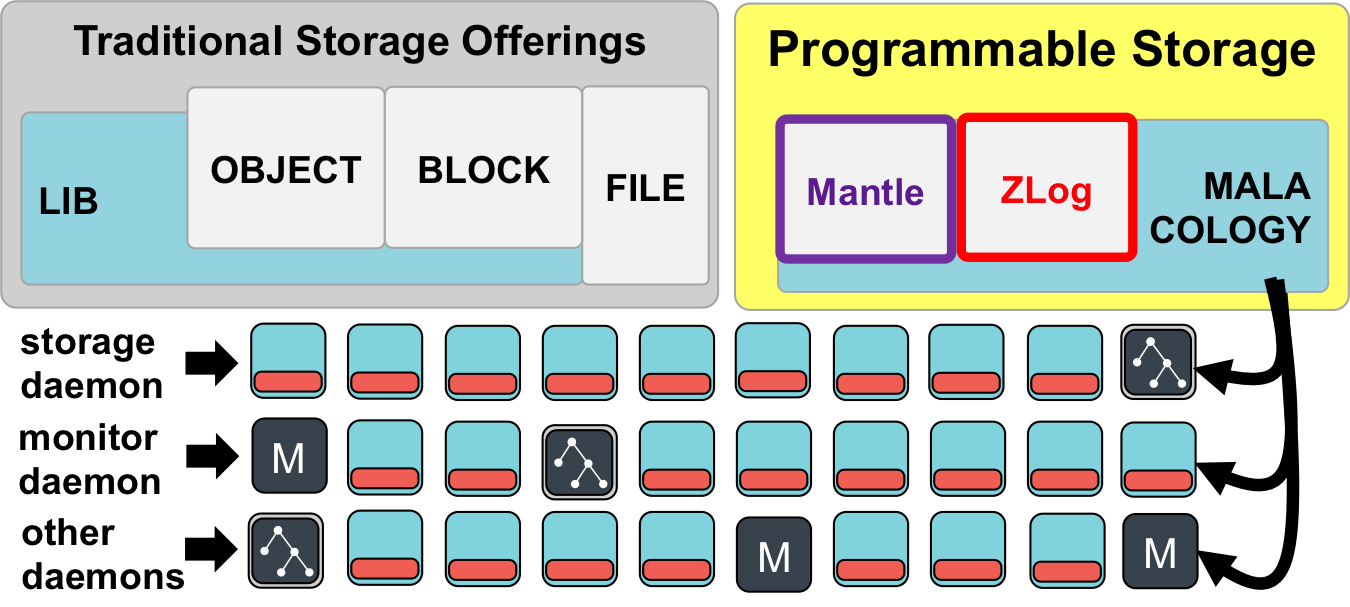
\includegraphics{figures/overview.png}
\caption{Scalable storage systems have storage daemons which store data,
monitor daemons (M) that maintain cluster state, and service-specific daemons
({\it e.g.}, file system metadata servers). Malacology enables the programmability of
internal abstractions (bold arrows) to re-use and compose
existing subsystems.  With Malacology, we add new services, ZLog and
Mantle, that sit alongside traditional user-facing APIs (file, block,
object).}\label{fig:overview}
\end{figure}

The evolutionary pressure placed on storage systems by these trends raises the
question of whether there are principles that storage systems designers can
follow to evolve storage systems efficiently, without jeopardizing years of
code-hardening and performance optimization efforts.  In this paper we
investigate an approach that focuses on identifying and exposing existing
storage system resources, services, and abstractions that in a generalized form
can be used to \emph{program} new services. By composing higher-level services
over existing abstraction one can reuse subsystems and leverage their
optimizations, established correctness, robustness, and efficiency. 

{\it \textbf{We define a programmable storage system}} to be a storage system
that facilitates the re-use and extension of existing storage abstractions
provided by the underlying software stack, to enable the creation of new
services via composition.  A programmable storage system can be realized by
exposing existing functionality (such as metadata services and synchronization
and monitoring capabilities) as interfaces that can be ``glued together'' in a
variety of ways using a high-level language. In contrast to programmable
storage, \emph{active storage} differs through its focus on the injection and
execution of code within a storage system or storage device. Programmable
storage differs from \emph{active storage}~\cite{riedel:vldb98}---the injection and
execution of code within a storage system or storage device---in
that the
former is applicable to any component of the storage system, while the latter
focuses at the data access level (i.e. inject and execute arbitrary code at the
I/O access layers). Given this contrast, we can say that active storage is an
example of how one internal component (the storage layer) is exposed in a
programmable storage system.

To illustrate the benefits and challenges of this approach we have designed and
evaluated Malacology, a programmable storage system that facilitates the
construction of new services by re-purposing existing subsystem abstractions of
the storage stack.  We build Malacology in Ceph, a popular open source software
storage stack.  We choose Ceph to demonstrate the concept of programmable
storage because it offers a broad spectrum of existing services, including
distributed locking and caching services provided by metadata servers,
durability and object interfaces provided by the backend object store, and
propagation of consistent cluster state provided by the monitoring service (see
Figure~\ref{fig:overview}). As we will show in this paper, Malacology is
expressive enough to provide the functionality necessary for implementing new
services. 
%Our contributions are:

% prototype programmable storage system that 
Malacology includes a non-exhaustive set of interfaces that can be used as
building blocks for constructing novel storage abstractions, including:

\begin{enumerate}

\item An interface for managing strongly-consistent time-varying \textbf{service
metadata}.

\item An interface for installing and evolving domain-specific, cluster-wide
\textbf{data interfaces}.

\item An interface for managing access to \textbf{shared resources} using a
variety of optimization strategies.

\item An interface for \textbf{load balancing} resources across the cluster.

\item An interface for \textbf{durability} that persists policies using the
underyling storage stack's object store.

\end{enumerate}

{\it \textbf{We implement two distributed services}} using Malacology to
demonstrate the feasibility of the programmable storage approach:

\begin{enumerate}

\item A high-performance distributed shared log service called ZLog, that is an
implementation of CORFU.~\cite{balakrishnan_corfu_2012}

\item An implementation of Mantle, the programmable load balancing
service~\cite{sevilla:sc15-mantle}

\end{enumerate}

The remainder of this paper is structured as follows. First, we describe and
motivate the need for programmable storage by describing current practices in
the open source community. Next we describe Malacology by presenting the
subsystems within the underlying storage system that we re-purpose, and briefly
describe how those system are used within Malacology (\S\ref{sec:malacology}).
Then we describe the services that we have constructed within the Malacology
framework (\S\ref{sec:services}), and evaluate our ideas within our prototype
implementation (\S\ref{sec:evaluation}).  We conclude by discussing related and future work.
% and
%conclude.

\section{Application-Specific Storage Stacks}
\label{sec:application-specifc-storage-stacks}

Building storage stacks from the ground up for a specific purpose results in
the best performance. For example, HDFS was designed specifically to serve
Hadoop's jobs, and uses techniques like exposing data locality and relaxing
POSIX constraints to to achieve application-specific I/O
optimizations.~\cite{CITEME}. Alternatively, general-purpose storage stacks are
built with the flexiblity to serve many applications by providing a variety of
interfaces and tunable parameters. Unfortunately, managing competing forces in
these systems is difficult and users want more control from the general-purpose
storage stacks without going as far as building their storage system from the
ground up.

To demonstrate this trend in storage systems we examine the state of
programmability in Ceph. Something of a storage swiss army knife, Ceph
simultaneously supports file, block, and object interfaces on a single
cluster~\cite{ceph_contributors_ceph_2010}. Ceph's Reliable Autonomous
Distributed Object Storage (RADOS) system is a cluster of storage devices
(OSDs) that provide Ceph with data durability and integrity using replication,
erasure-coding, and scrubbing~\cite{weil_rados_2007}. Ceph already provides
some degree of programmability; the OSDs support domain-specific object
interfaces that are implemented by composing existing low-level storage
interfaces that execute atomically. These interfaces are written in C++ and are
statically loaded into the system.

The Ceph community provides empirical evidence that developers are already
beginning to embrace programmable storage. Figure~\ref{fig:obj-int-dev-growth}
shows a dramatic growth in the production use of domain-specific interfaces in
the Ceph community since 2010. In that figure, classes are functional groupings
of methods on storage objects (e.g. remotely computing and caching the checksum
of an object extent).  What is most remarkable is that this trend contradicts
the notion that API changes are a burden for users.  Rather it appears that a
gap in existing interfaces are being addressed through ad-hoc approaches to
programmability. In fact, Table~\ref{table:objclasses} categorizes existing
interfaces and we clearly see a trend towards reusable services.

\begin{figure}[ht]
\centering
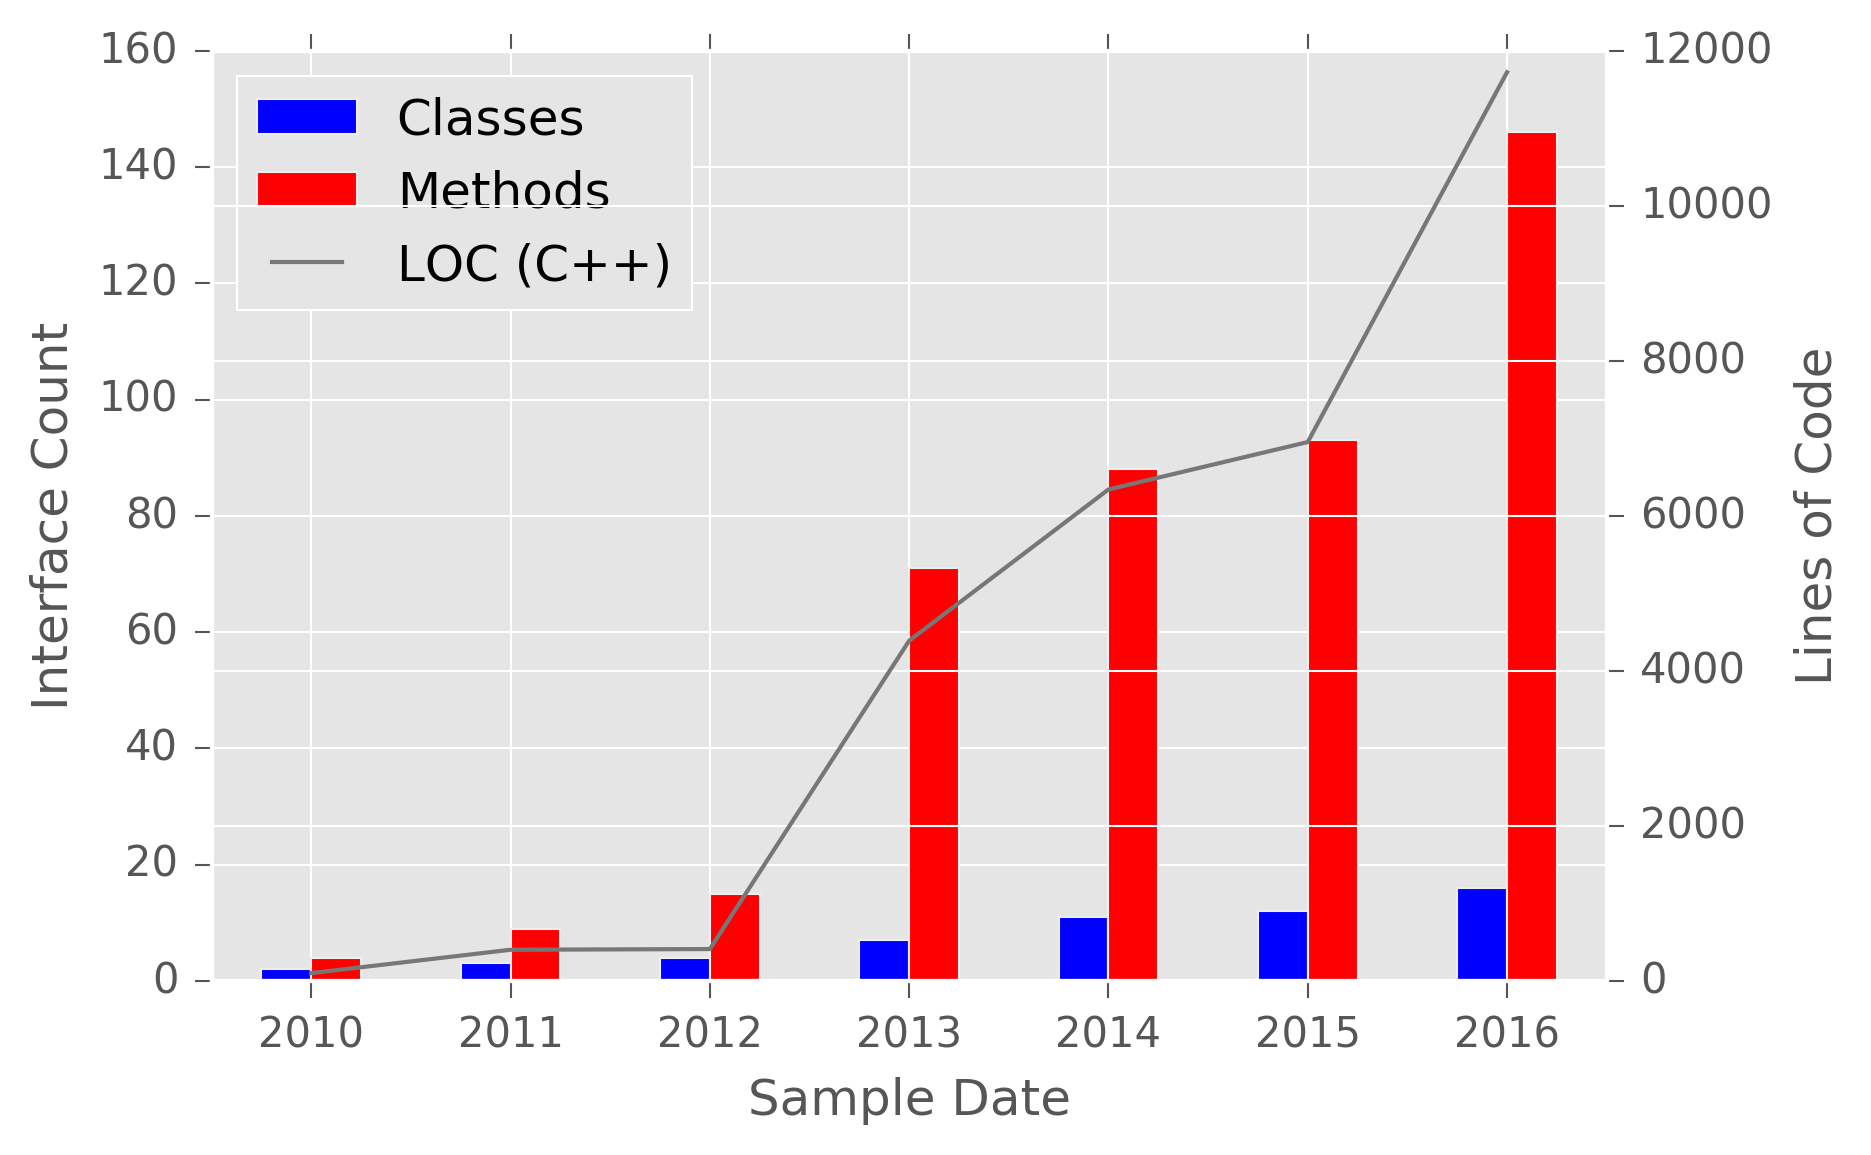
\includegraphics{figures/obj-int-dev-growth.png}
\caption{[\href{https://github.com/double-blind-submitter/osdi16}{source}]
Since 2010, the growth in the number of co-designed object storage interfaces
in Ceph has been accelerating. This plot is the number of object classes (a
group of interfaces), and the total number of methods (the actual API
end-points).}
\label{fig:obj-int-dev-growth}
\end{figure}

\begin{table}[ht]
\centering
  \begin{tabular}{l|l|l}
    Category & Example & \# \\ \hline
    Logging  & Geographically distribute replicas & 11 \\ \hdashline
    Metadata & Snapshots in the block device OR  & \multirow{2}{*}{74} \\
    Management & Scan extents for file system repair & \\ \hdashline
    Locking  & Grants clients exclusive access & 6 \\ \hdashline
    Other & Garbage collection, reference counting  & 4\\
\end{tabular}
\caption{A variety of object storage classes exist to expose interfaces
    to applications. \# is the number of methods that use these categories.
}
\label{table:objclasses}
\end{table}

The takeaway from Figure~\ref{fig:obj-int-dev-growth} is that programmers are
already trying to use programmability because their needs, whether they be
related to performance, availability, consistency, convenience, etc., are not
satisfied by the existing default set of interfaces. The popularity of the
custom object interface facility of Ceph could be due to a number of reasons,
such as the default algorithms/tunables of the storage system being
insufficient for the application's performance goals, programmers wanting to
exploit application-specific semantics, and/or programmers knowing how to
manage resources to improve performance. A solution based on
application-specific object interfaces is a way to work around the
traditionally rigid storage APIs because custom object interfaces give
programmers the ability to tell the storage system about their application: if
it is CPU or IO bound, if it has locality, if its size has the potential to
overload a single proxy node, etc.  The programmers know what the problem is
and how to solve it, but until the ability to modify object interfaces, they
had no way to express to the storage system how to handle their data.

Our approach is to expose more of the commonly used, code-hardened subsystems
of the underlying storage system as interfaces. The intent is that these
interfaces, which can be as simple as a redirection to the persistent data
store or as complicated as a strongly consistent directory service, should be
used and re-used in many contexts to implement a wide range of services. By
making programmability a `feature', rather than a `hack' or `workaround', we
help standardize a development process that now is largely ad-hoc.

\section{Challenges}
\label{sec:challenges}

Implementing the infrastructure for programmability into existing services and
abstractions of distributed storage systems is challenging, even if one assumes
that the source code of the storage system and the necessary expertise for
understanding it is available.  Some challenges include:

\begin{itemize}
	
\item Storage systems are generally required to be highly available so that any
complete restarts of the storage system to reprogram them is usually
unacceptable. 

\item Policies and optimizations are usually hard-wired into the services and
one has to be careful when factoring them out not to introduce additional bugs.
These policies and optimiations are usually cross-cutting solutions to concerns
or trade-offs that cannot be fully explored yet (as they relate to workload or
hardware). Given these policies and optimizations, decomposition of otherwise
orthogonal internal abstractions can be difficult or dangerous.

\item Mechanisms that are often only exercised according to hard-wired policies
and not in their full generality have hidden bugs that are revealed as soon as
those mechanisms are governed by different policies. In our experience
introducing programmability into a storage system proved to be a great
debugging tool.

\item Programmability, especially in live systems, implies changes that need to
be carefully managed by the system itself, including versioning and propagation
of those changes without affecting correctness.

\end{itemize}

To address these challenges we present Malacology. Malacology is both a
prototype for a programmable storage system and a design approach to evolve
storage systems efficiently and without jeopardizing years of code-hardening
and performance optimization efforts.  Although Malacology uses the internal
abstractions of the underlying storage system, including its subsystems,
components, and implementations, we emphasize that our system still addresses
the general challenges outlined above.

The main challenge of designing a programmable storage system is choosing the
right internal abstractions and picking the correct layers for exposing them.
In this paper, we do not present an exhaustive list of possible internal
abstractions nor do we contend that the abstractions we choose provide the best
trade-offs for all applications.  For example, if consensus is correctly
exposed one could implement high-level features like versioning, serialization,
or various flavors of strongly consistent data management on top; but perhaps a
low-level consensus interface is suited well for a particular set of
applications.  These questions are not answered in this paper and instead we
focus on showing the feasibility of building such a system, given advances in
the quality and robustness of today's storage stacks.

Malacology implements and demonstrates the ideas of programmable storage in
Ceph. We choose Ceph because it is a production quality system and because it
is open source. The large developer community ensures that code is
robust and the visibility of the code lets us expose any interface we want. In
the next section we describe the Ceph components that we expose as Malacology
interfaces.

\section{Malacology: A Programmable Storage System}
\label{sec:malacology}

\begin{table*}
\centering
\begin{tabular}{  l | l | l | l }
\multicolumn{4}{c}{\Large \textbf{Common Internal Abstractions}} \\
\multicolumn{4}{c}{} \\
\textbf{Abstraction}                    &
\textbf{Example in Production Systems}  &
\textbf{Example in Ceph}                &
\textbf{Provided Primitives}            \\ \hline
{\it Service Metadata}
  & Zookeeper/Chubby coordination~\cite{hunt_zookeeper_2010,website:chubby}
  & cluster state management~\cite{website:ceph-mon}
  & consensus \& consistency
  \\
{\it Shared Resource}
  & MPI collective IO, burst
  & POSIX metadata protocols
  & serialization \& batching
  \\
{\it Object \& Data}
  & Swift in situ storage/compute~\cite{website:zerocloud}
  & object interface classes~\cite{website:cls-lua}
  & transaction \& atomicity
  \\
Durability
  & S3/Swift interfaces (RESTful API)
  & object store library~\cite{weil_rados_2007}
  & interface to persistence
  \\
Load Balancing
  & VMWare's VM migration~\cite{vmware-drs,gulati:hotcloud2011-cloud-resource-management} 
  & migrate POSIX metadata~\cite{weil:sc2004-dyn-metadata}
  & migration \& sampling
  \\
\end{tabular}
\caption{The same ``internal abstractions" are common across large-scale
systems because they provide primitives that solve general distributed systems
problems.  Here we list examples of what these internal abstractions are used
for in ``production systems" and in Ceph.  Malacology provides these internal
abstractions as interfaces that higher level applications can use; {\it
italicized abstractions} are interfaces contributed in this paper.}
\label{table:examples}
\end{table*}

The guiding principle
is to re-use existing services and extend them so that these services can be
\emph{programmed}. We accomplish programmability of a service by exporting
bindings (or ``hooks'') for an interpreted programming language so that
programming can occur without having to restart the storage system (see also
below,~\S\ref{sec:durability}). 

There are multiple reasons that make Lua an attractive runtime for implementing
Malacology. Lua is a portable, embedded scripting language that offers superior
performance and productivity trade-offs, including a JIT-based implementation
that is well known for near native performance. Additionally, Lua has been used
extensively in game engines, and systems research \cite{neto:dls14-luaos},
including storage systems where it has been effectively used both on
\cite{grawinkel:pdsw2012-lua,watkins2013:bdmc13-in-vivo,geambasu_comet_2010}
and off \cite{sevilla:sc15-mantle} the performance critical path. Finally, the
flexibility of the runtime allows execution sandboxing in order to address
security and performance concerns.

We will now discuss the common subsystems used to manage storage system and how
Malacology makes them programmable.

\subsection{Service Metadata Interface}
\label{sec:mon}
\label{service-metadata}

% straw man example
Keeping track of the state of a distributed system is an essential part of any
successful service and a necessary component in order to diagnose and detect
failures, when they occur. This is further complicated by variable propagation
delays and heterogenous hardware in highly dynamic environments.

In the case of Ceph, a consistent view of cluster state among server daemons
and clients is critical to provide strong consistency guarantees to clients.
Ceph maintains cluster state information in per-subsystem data structures
called ``maps'' that record membership and status information.  A Paxos-based
monitoring service is responsible for integrating state changes into cluster
maps, responding to requests from out-of-date clients and synchronizing members
of the cluster whenever there is a change in a map so that they all observe the
same system state. As a fundamental building block of many system designs,
consensus abstractions such as Paxos are a common technique for maintaining
consistent data versions, and are a useful system to expose.

The default behavior of the monitor can be seen as a Paxos-based notification
system, similar to the one introduced in~\cite{burrows_chubby_2006}, allowing
clients to identify when new values (termed epochs in Ceph) are associated to
given maps.  While Ceph does not expose this service directly, a key-value
service designed for managing configuration metadata that is built on top of
the consensus engine is an example of a high-level service within Ceph that
re-uses existing abstractions.  While a key-value service is generally useful,
it doesn't provide many of the useful services hidden within the monitoring
framework that would be required for applications with more demanding
requirements, such as creating arbitrary maps with application-specific
semantics and interfaces. Since the monitor is intended to be out of
high-performance I/O paths, a general guideline is to make use of this
functionality infrequently and to assign small values to maps. 

\paragraph*{Malacology:} Malacology exposes a strongly-consistent view of
time-varying service metadata as a service rather than a hidden internal
component. Malacology provides a generic API for adding arbitrary values to
existing subsystem cluster maps. As a consequence of this, applications can
define simple but useful service-specific logic to the strongly-consistent
interface, such as authorization control (just specific clients can write new
values) or to trigger actions based on specific values (e.g. sanitize values).
The higher level services we implement in \S\ref{sec:services} make use of this
functionality to register, version and propagate dynamic code (Lua scripts) for
new object interfaces defined in storage daemons (\S\ref{object-data-interface}) and
policies in the load balancer \S\ref{malacology:mds}).  Using this service
guarantees that interface definitions are not only made durable, but are
transparently and consistently propagated throughout the cluster so that
clients are properly synchronized with the latest interfaces.

%And finally, it is important to not underestimate the importance of the
%preservation of the modifications that enable a new system service. In many
%(if not all) cases, interfaces defining access to data are just as important
%as the data itself by virtue of inherently providing structural context. Thus,
%all components of a system service must be kept to the same standards of
%protection as data in the system itself.

\subsection{Object I/O Interfaces}
\label{object-data-interface}

Briefly described in Section~\ref{sec:application-specifc-storage-stacks}, Ceph
supports the creation of application-specific object
interfaces~\cite{weil_rados_2007}. The ability to offload computation can
reduce data movement, and transactional interfaces can significantly simplify
construction of complex storage interfaces that require uncoordinated parallel
access. 

An object interface is a plugin structured in a similar way to that of an RPC
in which a developer creates a named function within the cluster that clients
may invoke. In the case of Ceph each function is implicitly run within the
context of an object specified when the function is called. Developers of
object interfaces express behavior by creating a composition of native
interfaces or other custom object interfaces, and handle serialization of
function input and output.  A wide range of native interfaces are available to
developers such as reading and write to a byte stream, controlling object
snapshots and clones, and accessing a sorted key-value database. These native
object interfaces may be transactionally composed along with application
specific logic to create interfaces with a rich set of semantics.  An example
is the use of a read-modify-write operation to perform consistent object
updates across the byte stream and key-value database interfaces without
relying on complex client-driven concurrency control.

\begin{figure}[htbp]
\centering
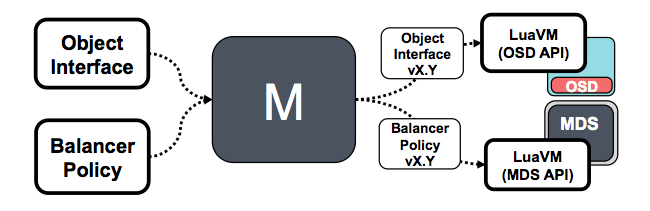
\includegraphics{figures/implementation.png}
\caption{Malacology re-uses Ceph subsystems to allow users to dynamically
define new object/data interfaces and load balancing policies. It achieves this
by extending the object storage daemon (OSD) and metadata server daemon (MDS)
subsystems with an embedded Lua VM.  It uses the of the strongly-consistent
service metadata interface to propogate the object interfaces and versions
across the cluster.
\label{fig:implementation}} \end{figure}

\paragraph*{Malacology:} The implementation of Ceph's object abstraction,
although powerful, does not readily support programmability. Supporting only
C/C++ for object interface developers, Ceph requires distribution of compiled
binaries for the correct architecture, adding a large barrier of entry for
developers and system administrators. Second, having no way to dynamically
unload modules, any changes require a full restart of a storage daemon which
may have serious performance impacts due to loss of cached data. And finally,
the security limitations of the framework limit the use of object interfaces to
all but those with administrative level access and deep technical expertise.

To address these concerns, Malacology takes advantage of Lua extensions
contributed by the Ceph community. This allows new object interfaces to be
dynamically loaded into the system and modified at runtime, resulting in a
object storage API with economy of expression, which at the same time provides
the full set of features of the base object class. New object interfaces that
are expressed in thousands of lines of code can be implemented in approximately
an order of magnitude less code~\cite{geambasu_comet_2010}. While the use of
Lua does not prevent deployment of malicious code, certain types of coding
mistakes can handled gracefully, and access policies are used to restrict the
feature to trusted users.

All of these modifications work in tandem to implement the desired behavior,
and are typically co-designed together such that each depends on the other to
behave as expected. 

\subsection{Distributed Metadata Interfaces}
\label{malacology:mds}

The distributed metadata service in Ceph provides clients with a POSIX file
system abstraction~\cite{weil:sc2004-dyn-metadata}. In general, distributed
file systems protect resources by providing hierarchical indexing and
distributed locking services.  In Ceph, the locking service implements a
capability-based system that expresses what data and metadata clients are
allowed to access as well as what state they may cache and modify locally.
While designed for a fixed file abstraction, indexing, locking, and caching are
all common services that are useful to a broad spectrum of applications.
Distributed applications that share centralized resources (e.g. a database or
directory) face similar challenges which are often solved using
application-specific sharding. 

Ceph also addresses the challenge of balancing metadata load with a separate
metadata cluster. This cluster uses load balancing policies to migrate
directory inodes around the cluster to alleviate overload at single nodes. The
policies use metrics based on system state (e.g.  CPU and memory utilization)
and statistics collected by the cluster (e.g. the popularity of an inode). Ceph
uses dynamic subtree partitioning to move variable sized namespace
subtrees~\cite{weil:sc2004-dyn-metadata}. These units can be shipped anywhere
(i.e., to any metadata server of any capacity) at any time for any reason. The
original balancer was designed with hard-coded policies and tunables.

%The metadata cluster moves units of the namespace called directory fragments
%and assigns them to servers using its own metadata load balancer. It then uses
%a hard-coded policy to balance these fragments using a scalarized load metric
%based on CPU, workload, and file system operation metrics. Although the CephFS
%balancer has been shown to be complicated, its complexity is justifiable.
%Having the flexibility to choose what to move, where to move it, and how much
%to move is very powerful. The problem is that it is difficult to pick a
%one-size-fits-all policy, system administrators may want to partition load
%based on SLAs, or applications are better equipped to make these decisions,
%etc. -- but we choose instead to expose a balancing API at strategic points in
%the balancing logic using Lua hooks. ~\cite{sevilla:sc15-mantle}. 

\paragraph*{Malacology:} interfaces are added in strategic spots in the
metadata service for guarding shared resources, defining new file types,
and load balancing.

{\bf Shared resource interface.}
The metadata service manages client sessions, allowing clients to obtain locks
(e.g. file byte ranges), and capabilities (e.g. to cache file data). Clients
and metadata servers use a cooperative protocol in which clients voluntarily
release resources back to the metadata service in order to implement sharing
policies. While the current policy for sharing access and voluntarily
releasing resources is largely best-effort, Malacology supports generalized
policies between metadata servers and clients that can be used to implement 
fairness or priority.

{\bf File type interface.} The metadata service manages a POSIX file system
hierarchy where files and directories are represented as inode data structures
and expose a POSIX file interface. Application that manage large amounts of
metadata (e.g. users or database snapshots) often require a naming service. We
allow new inode types to be defined such that applications can create
domain-specific interfaces to inodes that may modify locking and capability
policies. We will show this is used in Section~\ref{sec:seq} when we discuss a
distributed shared-log built on Malacology.

{\bf Load balancing interface.} Mantle~\cite{sevilla:sc15-mantle}, a
programmable metadata load balancer, has been implemented on Malacology so that
its infrastructure can enjoy all the properties of existing internal
abstractions.  The load balancing logic is intact but the infrastructure has
been improved to safely load, manage, and persist its load balancing policies.
Composing Mantle using the service metadata and durability interfaces, Mantle
can safely version balancer policies, save balancer policies in the backend
object store and centralize warnings/errors. When combined with file types,
load balancing policies can express a variety of rules such as multi-tentant
and multi-application balancing.

%{\bf Policy management.} A new interface is added to the metadata service
%subsystem using the monitoring framework to support management of interfaces.
%This ensures that the correct balancer version is consistently distributed and
%verified on all MDS nodes. Policies are also durably saved with Ceph's
%replication and redundancy.

%These problems are general, distributed systems load balancing problems and
%share many of the same properties as the POSIX metadata
%wall~\cite{alam:pdsw2011-metadata-scaling,ghemawat:sosp2003-gfs,hildebrand:msst2005-pnfs,weil_ceph_2006,welch:fast2008-panasas,shvachko:login2012-hdfs-scalability}.
%Many distributed file systems decouple metadata and data I/O so that these
%services can scale independently. Despite this optimization, scaling the
%metadata services is still difficult because metadata accesses impose small
%and frequent requests on the underlying storage
%system~\cite{roselli:atec2000-FS-workloads}. Many techniques for designing the
%metadata services have been proposed to accommodate this workload:
%Lustre~\cite{konstantinos:pdsw2014-lustre-metadata},
%GFS~\cite{ghemawat:sosp2003-gfs}, and
%HDFS~\cite{shvachko:login2012-hdfs-scalability} keep all metadata on one
%server; GIGA+~\cite{patil:fast2011-giga}, IndexFS~\cite{ren:sc2014-indexfs},
%Lazy Hybrid~\cite{brandt:msst2003-lh}, GPFS~\cite{schmuck:fast2002-gpfs}, and
%pNFS~\cite{hildebrand:supercomputing2006-pNFS} hash the file system namespace
%across a dedicated cluster and cache metadata;
%Panasas~\cite{welch:fast2008-panasas} and
%CephFS~\cite{weil:sc2004-dyn-metadata} use subtree partitioning to carve up
%the namespace and distribute it across a cluster.
%
%Both the object and balancer interfaces define functions and attach them
%to the core Lua sandbox. For example, the Lua object storage interface
%class attaches data, extended attribute, object map, and object version
%functions, to the Lua core functions, as shown in Figure
%\ref{fig:cls-osd-mds}. The advantages of this is that we avoid
%duplicating code, we provide a framework for putting Lua code in other
%parts of the system, and we remove components and APIs that are too
%integrated with the OSD.

%To facilitate the use of Lua in both the MDS and OSD, we modularize the LuaVM
%in a core sandbox wrapper and link against it, as shown in
%Figure~\ref{fig:cls-osd-mds}. This core Lua wrapper contains just the
%dependencies, symbols, and functions, needed to run the Lua VM and strips away
%all the functionality inherent to object classes (like placement group
%filters, cryptography functions, object metadata,  object data, object
%extended attributes, and object versions). Some functions of Ceph's more
%helpful subsystems, like the logging facilities for the daemons, were re-used
%in the MDS.  With this scheme, The OSD will dynamically open the shared
%library created by Lua object interface shared library while the MDS will
%dynamically open the Lua balancer interface shared library; both shared
%libraries will the Lua core.

%{\bf File Types.} We leverage the same active and typed storage module
%presented in DataMods~\cite{watkins_datamods_2012} to assign state and a set of
%functions to a file (stored in the inode). This is valuable for
%metadata load balancing so that certain types of files can have a higher
%priority when making balancing decisions.

%\begin{figure}[h]
%\centering
%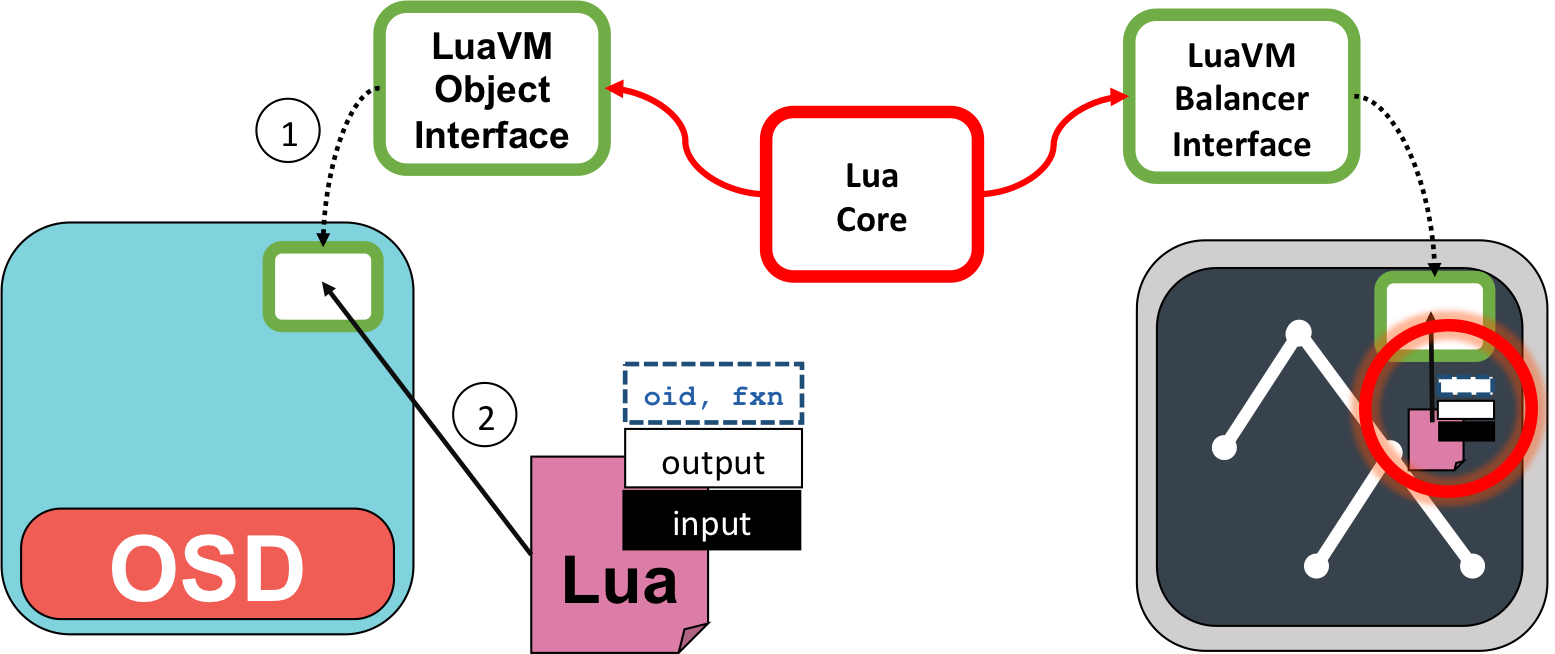
\includegraphics{figures/cls-osd-mds.png}
%\caption{To generalize the LuaVM for use in both the OSD and MDS,
%Malacology detaches the core functionality into a Lua core module. The
%VM is dynamically loaded first (1) and then interfaces can execute (2).
%\label{fig:cls-osd-mds}}
%\end{figure}

% Straw man example
%Migrating resources is an important part of load balancing but understanding
%the effects of different configurations and parameters is difficult. Systems
%already virtualize and migrate memory; soon systems will be able to migrate
%other resources, like CPU, disk, and memory. Figuring out how, when, and where
%to move these resources depends on complex metrics like utilization,
%configuration, and workload.

%These hooks embed Lua code in the MDS using the OSD subsystems. By re-using
%the OSD interface classes, the MDS gets the safety and robustness of loading
%dynamic code (including graceful failures and helpful errors), the ease of
%transferring state between object interfaces and the OSD internals,
%integration with testing and correctness suites, and \texttt{struct}s for
%interface data and handlers. 

\subsection{Durability Interface}
\label{sec:durability}

Ceph provides storage by striping and replicating data across
RADOS~\cite{weil_rados_2007}, the reliable distributed object store. RADOS uses
many techniques to ensure that data is not corrupted or lost, such as erasure
coding, replication, and data scrubbing.  Furthermore, many of these features
are implemented using a peer-to-peer protocol that allows object storage
devices to operate autonomously without a centralized coordinator.  For
example, when the number of placement groups change, the OSDs re-balance and
re-shard data in the background in a process called placement group splitting
in which OSDs communicate directly with each other to coverage on a new state.
In order to reduce load on the monitoring service, Ceph OSDs use a gossip
protocol to efficiently propagate changes to cluster maps throughout the
system, and autonomously initiate recovery mechanisms when failures are
discovered.

\paragraph*{Malacology:} Metadata service policies and object storage
interfaces are stored durability within RADOS and managed by storing references
with the object maps. Since the cluster already propagates a consistent view of
these data structures, we use this service to automatically install interfaces
in OSDs, and install policies within the MDS such that clients and daemons are
synchronized on correct implementations without restarting.

\section{Services Built on Malacology}
\label{sec:services}
\label{services-built-on-malacology}

\label{services}
\begin{table}
\centering
\begin{tabular}{  l | l | l }
\textbf{Service}              &
\textbf{Used to...}           &
\textbf{Malacology Interface} \\ \hline
Mantle & load balance metadata     & Load Balancing  \\
       & agree on current balancer & Service Metadata\\
       & control client write lock & Shared Resource \\
       & persist policy logic      & Durability      \\ \hline
ZLog   & implement CORFU           & Object \& Data  \\ 
       & install ZLog interfaces   & Service Metadata\\
       & persist log entries       & Durability      \\ \hline
ZLog   & load balance sequencers   & Load Balancing  \\
Seqr.  & manage access to log tail & Shared Resource \\ 
\end{tabular}
\caption{Mantle and ZLog are built using Malacology interfaces so they inherit the
robustness of the subsystems of the underlying stack.}
\label{table:implementation}
\end{table}

In this section we describe two services built on top of Malacology. The first
is Mantle, a framework for dynamically specifying metadata load balancing
policies. The second system, ZLog, is a high-performance distributed shared-log.
In addition to these services, we'll demonstrate how we combine ZLog and Mantle
to implement service-aware metadata load balancing policies.

\subsection{Mantle: Programmable Load Balancer}
\label{sec:mantle}

Mantle is a programmable load balancer that separates the metadata balancing
policies from their mechanisms. Administrators inject code to change how the
metadata cluster distributes metadata. In ~\cite{sevilla:sc15-mantle} the
authors showed how using Mantle, one can implement a single node metadata
service, a distributed metadata service with hashing, and a distributed
metadata service with dynamic subtree partitioning. 

The original implementation was ``hard-coded" into Ceph and lacked robustness
(no versioning, durability, or policy distribution).  Re-implemented using
Malacology, Mantle now enjoys (1) the versioning provided by the metadata
service interface provided by the monitor daemons and (2) the durability and
distribution provided by Ceph's reliable object store.  

\subsubsection{Versioning Balancer Policies}

Ensuring that the version of the current load balancer is consistent across the
physical servers in the metadata cluster was ignored in the original
implementation. The user had to set the version on each individual server and
it was trivial to make the version inconsistent. Maintaining a consistent
version is important for balancing policies that are cooperative in which local
decisions are made assuming properties about other instances of the same
policy.

With Malacology, Mantle stores the version of the current load balancer in the
Ceph service metadata interface. The version of the load balancer corresponds
to an object name in the balancing policy. Using the service metadata interface
ensures that all metadata servers use the same version of the load balancer. As
a result, the policy version inherits the consistency of Ceph's internal
monitor daemons.

The user changes the version of the load balancer using a new CLI command: \\

\noindent \texttt{\$> ceph fs\ set\ lua\_balancer\_class\ \textless{}version\textgreater{}}

%There are Ceph components that are obstacles to this approach, namely the size
%of the  MDS map, API changes, and security. The Ceph engineers want to avoid
%using the maps to exchange information; the maps should be lightweight and fast
%because the MONs need to be able to version MDS cluster state quickly. API
%changes can also be a burden, especially for the MDS map, since all clients
%need to have the same version of the CephFS library in order to properly
%interact with CephFS. Finally, Ceph tries to avoid injecting strings into the
%cluster because they are insecure and buggy. 

\subsubsection{Making Balancer Policies Durable}

The load balancer version described above corresponds to the name of an object
in RADOS that holds the actual Lua balancing code.  When MDS nodes start
balancing load, they first check the latest version from the MDS map and
compare it to the balancer they have loaded. If the version has changed, they
dereference the pointer to the balancer version by reading the corresponding
object in RADOS. This is in contrast to the original balancer which stored load
balancer code on the local file system -- a technique which is unreliable and
may result in silent corruption.

The balancer pulls the Lua code from RADOS synchronously; asynchronous reads
are not possible because of the architecture of the MDS. The synchronous
behavior is not the default behavior for RADOS operations, so we achieve this
with a timeout: if the asynchronous read does not come back within half the
balancing tick interval the operation is cancelled and a Connection Timeout
error is returned. By default, the balancing tick interval is 10 seconds, so
Mantle will use a 5 second second timeout.

This design allows Mantle to immediately return an error if anything
RADOS-related goes wrong.  We use this implementation because we do not want to
do a blocking OSD read from inside the global MDS lock. Doing so would bring
down the MDS cluster if any of the OSDs are not responsive.

Storing the balancers in RADOS is only possible because we use Lua as the
language for writing balancer code. If we used a language that needs to be
compiled, like the C++ object classes in the OSD, we would need to ensure
binary compatibility, which is complicated by different operating systems,
distributions, and compilers.

\subsubsection{Logging, Debugging, and Warnings}

In the original implementation, Mantle would log all errors, warnings, and
debug messages to a log stored locally on each MDS server. To get the simplest
status messages or to debug problems, the user would have to log into each MDS
individually, look at the logs, and reason about causality and ordering.

With Malacology, Mantle re-usues the centralized logging features of the
monitoring service. Important errors, warnings, and info messages are collected
by the monitoring subsystem and appear in the monitor cluster log so instead of
users going to each node, they can watch messages appear at the monitor.
Messages are logged sparingly, so as not to spam the monitor with frivolous
debugging but important events, like balancer version changes or failed
subsystems show up in the centralized log.

\subsection{ZLog: A Fast Distributed Shared Log}
\label{sec:zlog}

The second service implemented on Malacology is ZLog, a high-performance
distributed shared-log that is based on the CORFU
protocol~\cite{balakrishnan_corfu_2012}. A shared-log is a general, yet
powerful abstraction used to construct distributed systems, such as
cloud-based metadata management~\cite{balakrishnan:sosp13} and elastic database
storage engines~\cite{bernstein:cidr11,bernstein:vldb11,bernstein:sigmod15}.
However, existing implementations that rely on consensus algorithms such as
Paxos funnel I/O through a single point introducing a bottleneck that restricts
throughput.  In contrast, the CORFU protocol is able to achieve high throughput
using a network counter service, called a \emph{sequencer}, that is used to
decouple log position assignment from log I/O.

While a full description of the CORFU system is beyond the scope of this
paper, we briefly describe the custom storage device interface, sequencer
service, and recovery protocol, and how these services are instantiated in the
Malacology framework.

\subsubsection{Sequencer}
\label{sec:seq}

High-performance in CORFU is achieved using a sequencer service that assigns
log positions to clients by reading from a volatile, in-memory counter which
can run at a very high throughput and at low latency. Since the sequencer
is centralized, ensuring serializability in the common case is trivial.  The
primary challenge in CORFU is handling the failure of the sequencer in a way
that preserves correctness. Failure of the sequencer service in CORFU is
handled by a recovery algorithm that recomputes the new sequencer state using
an application-specific custom storage interface to discover the tail of the
log, while simultaneously invalidating stale client requests using an
epoch-based protocol.

{\bf Sequencer interface.} The sequencer resource supports the ability to
\emph{read()} the current tail value as well as get the \emph{next()} position in
the log which also atomically increments the tail position.
We implement the sequencer service in Malacology as an application-specific
file type that associates a small amount of metadata, including the 64-bit log
tail position, to the inode state managed by the Ceph metadata service. Since
a sequencer is associated with a unique log, this approach has the added
benefit of allowing the metadata service to also handle naming, by
representing each log service instance within the standard POSIX hierarchical
namespace. The primary challenge in mapping the sequencer resource to the
metadata service is handling serialization correctly to maintain the global
ordering provided by the CORFU protocol.

Initially we sought to directly model the sequencer service in Ceph as a
non-exclusive, non-cacheable resource, forcing clients to perform a round-trip
access to the resource at the authoritative metadata server for the sequencer
inode.  Interestingly, we found that the capability system in Ceph uses a
strategy to reduce metadata service load by allowing clients that open a
shared file to temporarily obtain an exclusive cached copy of the resource,
resulting in a round-robin, best-effort batching behavior. When a single
client is accessing the sequencer resource it is able to increment the
sequencer locally. Any competing client cannot query the sequencer until the
metadata service has granted it exclusive access.

While unexpected, this discovery allowed us to explore an implementation
strategy that we had not previously considered. In particular, for bursty
clients, and clients that can tolerate increased latency, this mode of
operation may allow a system to achieve much higher throughput than a system
with a centralized sequencer service.  We utilize the programmability of the
metadata service to define a new policy for handling capabilities that controls
the amount of time that clients are able to cache the sequencer resource. This
allows an administrator or application to control the trade-off between latency
and throughput beyond the standard best-effort policy that is present in Ceph
by default. 

In Section~\ref{evaluation} we quantify the trade-offs of throughput and
latency for an approach based on a round-robin batching mode, and compare this
mode to one in which the metadata server mediates access to the sequencer state
when in it is being shared among multiple clients. Quantifying these trade-offs
should provide administrators with guidelines for setting the tunables for
different ``caching" modes of the sequencer.

{\bf Balancing policies.}
As opposed to the batching mode for controlling access to the sequencer
resource, more predictable latency can be achieved by treating the sequencer
inode as a shared non-cacheable resource, forcing clients to make a round-trip
to the metadata service. However, the shared nature of the metadata service
may prevent the sequencer from achieving maximum throughput. To provide a
solution to this issue we have taken advantage of the programmability of the
metadata service load balancing to construct a service-specific load balancing
policy. As opposed to a generic balancing policy that may strive for uniform
load distribution, a ZLog-specific policy may utilize knowledge of inode types
to migrate the sequencer service to provisioned hardware during periods of
contention or high demand.

\subsubsection{Storage Interface}

The storage interface is a critical component in the CORFU protocol. Clients
independently map log positions that they have obtained from the sequencer
service (described in detail in the next section) onto storage devices, while
storage devices provide an intelligent \emph{write}-once, random \emph{read}
interface for accessing log entries. The key to correctness in CORFU lies with
the enforcement of up-to-date epoch tags on client requests; requests tagged
with out-of-date epoch values are rejected, and clients are expected to
request a new tail from the sequencer after refreshing state from an auxiliary
service.  This mechanism forms the basis for sequencer recovery.

In order to repopulate the sequencer state (i.e. the cached, current tail of
the log) during recovery of a sequencer, the maximum position in the log must
be obtained. To do this, the storage interface exposes an additional
\emph{seal} method that atomically installs a new epoch value and returns the
maximum log position that has been written.

Since the sequencer servivce does not resume until the recovery process has
completed, there cannot be a race with clients appending to the log, and the
immutability of the log allow reads to never block during a sequencer failure.
Recovery of the sequencer process itself may be handled in many ways, such as
leader election using an auxiliary service such as Paxos. In our
implementation, the recovery is the same (and is inherited from) the Ceph
metadata service. Handling the failure of a client that holds the sequencer
state is similar, although a timeout is used to determine when a client should
be considered unavailable.

\section{Evaluation}
\label{sec:evaluation} 

%We wanted to implement CORFU and we had two choices: build it from the ground
%up or do it on top of Malacology. To show the feasability of building on
%Malacology our evaluation focuses on the 

Our evaluation demonstrates the feasibility of building new service
abstractions atop programmable storage, focusing on the performance of the
internal abstractions exposed by Malacology and used to construct the Mantle
and ZLog services. We also discuss latent capabilities we discovered in this
process that let us navigate different trade-offs within the services
themselves. First, we benchmark scenarios with high sequencer contention by
examining the interfaces used to map ZLog onto Malacology; specifically, we
describe the sequencer implementation and the propagation of object and data
interfaces interfaces.  Next, we benchmark scenarios in which the storage
system manages multiple logs by using Mantle to balance sequencers across a
cluster.

% should save this for future work, otherwise it undercuts the eval.
%Detailed system-wide performance measurements and analysis is forthcoming for
%both Mantle and ZLog, as we try to find the best metadata balancing policies
%and physical design implementation trade-offs.  

Since this work focuses on the programmabilty of Malacology, the goal of this
section is to show that the components and subsystems that support the
Malacology interfaces provide reasonable relative performance, as well as to
give examples of the flexibility that Malacology provides to programmers.

%As we search for the best metadata balancing policies
%and physical design implementation trade-offs,
%we plan to rel

\subsection{Mapping ZLog onto Malacology}
\label{sec:mapping-zlog-onto-malacology}

We evaluate Malacology by exploring one possible mapping of the ZLog
implementation of CORFU onto Ceph in which we re-use (1) the metadata service
to manage naming and synchronization of the sequencer resource by treating the
resource as an inode, and (2) the monitoring sub-subsystem to distribute and
install application-specific I/O interface required of the CORFU protcool. In
Section~\ref{sec:zlog-balancing} we then demonstrate how the re-use of the inode
abstraction for implementing the sequencer resource enables load balancing policies
to migrate the sequencer resource in heavy-load situation.

\subsubsection{Sequencer Implementation}
\label{sec:sequencer-implementation}

We evaluate the feasibility of using the metadata service to implement a
seqeuencer resource that is responsible for maintaining a total ordering of
the log. Clients contact the sequencer to obtain the tail of the log and then
independently initiate I/O, thus we measure both the throughput and latency of
obtaining new tail positions which inherently bound client append performance.

The sequencer is implemented as a custom file type in which the sequencer
state (a 64-bit integer) is embedded in the inode of a file representing the
sequencer. A total ordering of the log is imposed by the re-use of the
capability service that can be used to grant exclusive access of inode state
to clients. The metadata service is responsible for maintaining exclusivity
and granting access. Figure~\ref{fig:capdelay-quota-behavior} (a) shows the
behavior of the system in which a best-effort policy is used.  The two colors
represent points in time that the clients were able to access the resource.
The best-effort policy provides interleaving a high degree of interleaving
between clients but the system spends a large portion of time re-distributing
the capability, reducing overall throughput.

In order to control the performance of the system we implement a
policy that (1) restricts the length of time that a client may maintain
exclusive access and (2) limits the number of log positions that a client may
generate without yielding to other clients waiting for access. The behavior of
these two modes is illustrated in Figures~\ref{fig:capdelay-quota-behavior}
(b) and (c), respectively.

\begin{figure}[h]
\centering
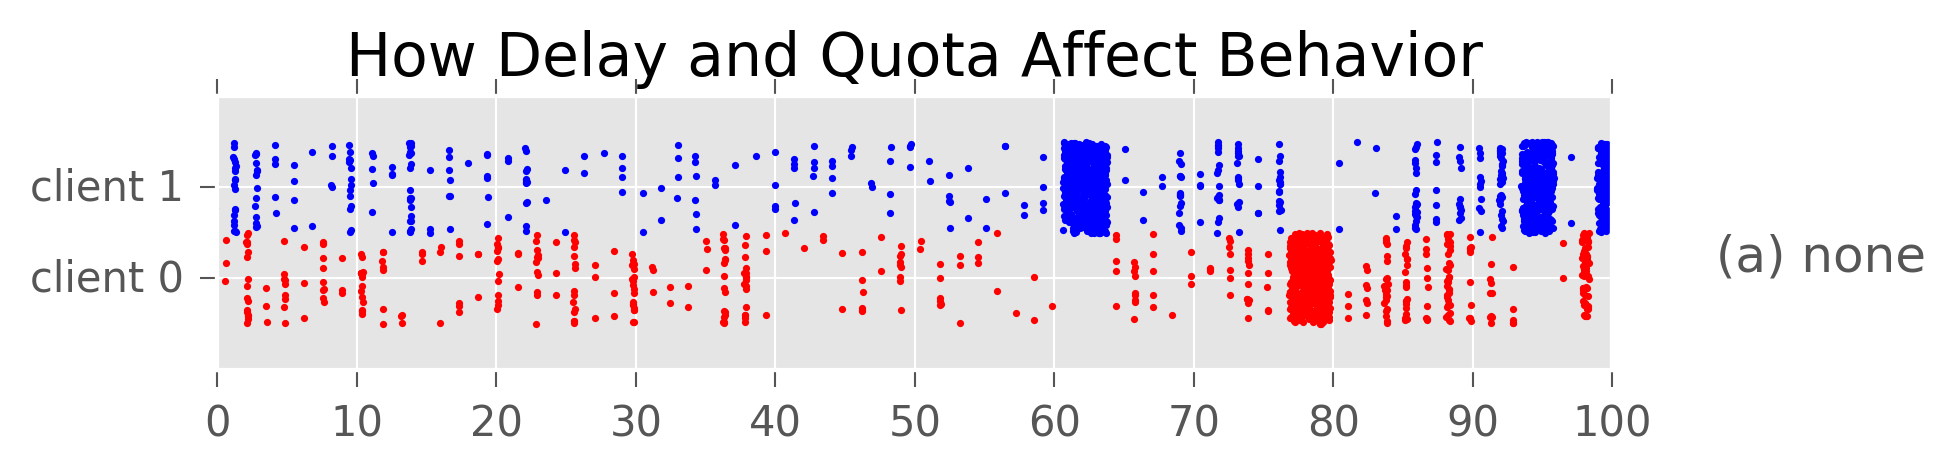
\includegraphics{figures/capdelay-quota-behavior-a.png}
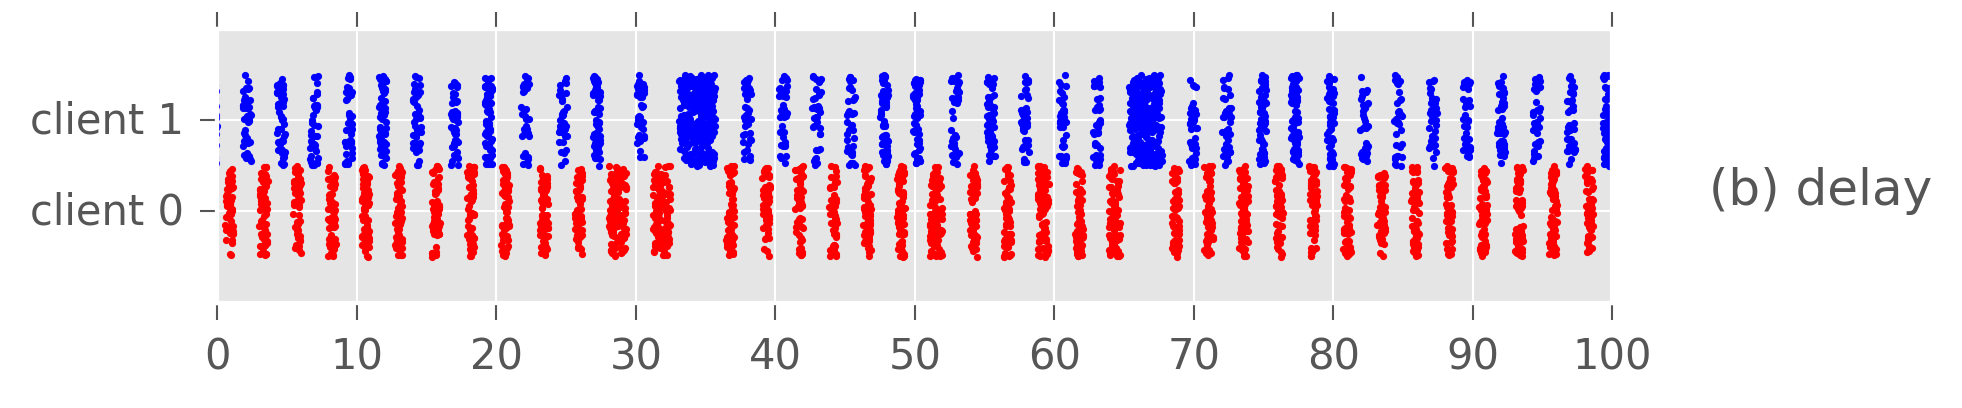
\includegraphics{figures/capdelay-quota-behavior-b.png}
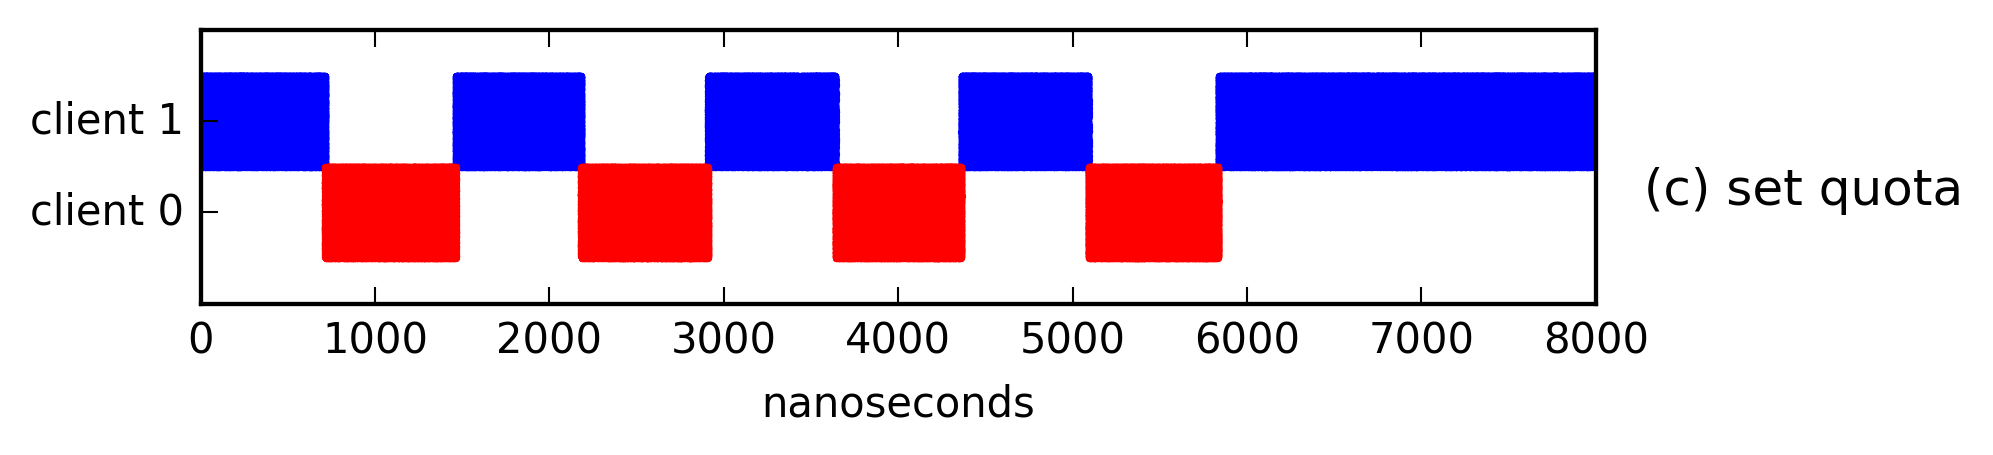
\includegraphics{figures/capdelay-quota-behavior-c.png}
\caption{Each dot in these graphs is an individual request and they are spread
randomly along the \(y\) axis. The default behavior (``None") shows
unpredictable performance, ``delay" lets each client hold the lease longer, and
``quota" gives each client the lease for a certain number of operations. Delay
improves latency and fairness while quota maximizes throughput.}
\label{fig:capdelay-quota-behavior}
\end{figure}

Figure~\ref{fig:captp} demonstrates a configurable trade-off between
throughput and latency. In the experiment two clients are run each with a
fixed 0.25 second maximum reservation on the capability, and we vary the size
of the log position quota running each configuration for two minutes. The
total operations per second is the combined throughput of the two clients, and
the average latency is number of microseconds required to obtain a new log
position. With a small quota more time is spent exchanging exclusive access,
while a large quota reservation allows clients to experience a much lower
latency because they uncontended access for a longer period of time.


\begin{figure}[h]
\centering
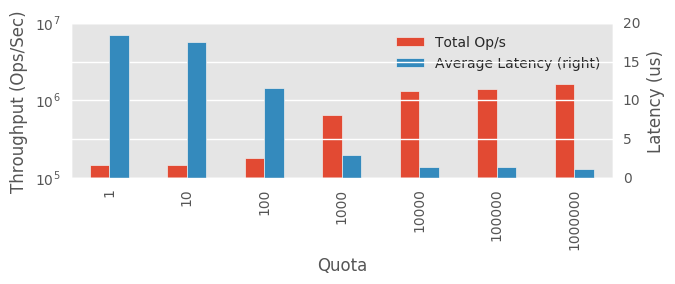
\includegraphics{figures/tradeoff.png}
\caption{[\href{https://github.com/double-blind-submitter/osdi16}{source}]
Sequencer throughput by re-using various services.  The highest performance is
achieved using a single client with exclusive, cacheable privilege. Round-robin
sharing of the sequencer resource is affected by the amount of time the
resource is held, with best-effort performing the worst.}
\label{fig:captp}
\end{figure}

To get a better picture of latency, Figure~\ref{fig:capcdf} shows the CDF of
latency for each client in all experiment configurations. At the 99th
percentile clients accessed the sequencer is less than a millisecond. The CDF
is cropped at the 99.999th percentile due to large outliers that we believe
occur in instances in which the MDS is performing I/O while it is in the
process of re-distributing the capability to another client.

\begin{figure}[h]
\centering
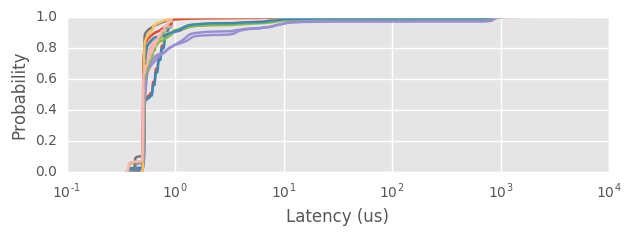
\includegraphics{figures/caps-delay-latency.png}
\caption{
The latency distribution shows that if the clients hold their capabilities longer,
performance decreases. Changing the delay via policy can help the sequencer and
clients strike a balance between throughput and latency.}
\label{fig:capcdf}
\end{figure}

We have shown how exposing the internal capability management service allows
users to navigate latency and throughput tradeoffs.  Other approaches to
designing the sequencer service also exist, such as using a centralized
service in which each access is a network round-trip. In contrast to the
mechanism we explored which is appropriate for clients with bursty workloads,
it may be easier to provide predictable performance using a centralized
service, and we will be exploring in the future how this can be achieved using
the capability system.

\subsubsection{Interface Propagation}

Domain-specific data interfaces (Section~\ref{object-data-interfaces}) allow
co-design between applications and the storage system. Malacology supports
custom object interfaces in RADOS that require interface implementations to
be installed on the storage devices in the system, supporting the evolution of
interfaces through automatic system-wide versioning and installation through
the service metdata interface (Section~\ref{service-metadata}). We evaluate
the performance of installing a new version of an interface in the cluster,
which is an important metric for applications that are designed with
frequently evolving interfaces.

We demonstrate the feasibility of utilizing the Ceph monitoring sub-system by
evaluating the performance of installing and distributing interface updates.
Figure~\ref{fig:propdelay} shows the CDF of the latency of interface updates.
The interfaces are Lua scripts embedded in the cluster map and distributed
using a peer-to-peer gossip protocol.  The latency is defined as the elapsed
time following the Paxos proposal for an interface update until each OSD makes
the update live (the cost of the Paxos proposal is configurable and is
discussed below). The latency measurements were taken on the nodes running
Ceph server daemons, and thus exclude the client round-trip cost. In each of
the experiments 1000 interface updates were observed.

Figure~\ref{fig:propdelay} shows the lower bound cost for updates in a large
cluster. In the experiment labeled "120 OSD (RAM)" a cluster of 120 OSDs (10
OSDs x 12 servers) using an in-memory data store were deployed, showing a
latency of less than 54 ms with a probability of 90\% and a worst case latency
of 194 ms. These costs demonstrate the penality of distributing the interface
in a large cluster. In practice the costs include, in addition to cluster-wide
propagation of interface updates, the network round-trip to the
interface management service, the Paxos commit protocol itself, and other factors
such as system load. By default Paxos proposals occur periodically with a 1
second interval in order to accumulate updates. In a minimum, realistic quorum
of 3 monitors using HDD-based storage, we were able to decrease this interval
to an average of 222 ms.

\begin{figure}[h]
\centering
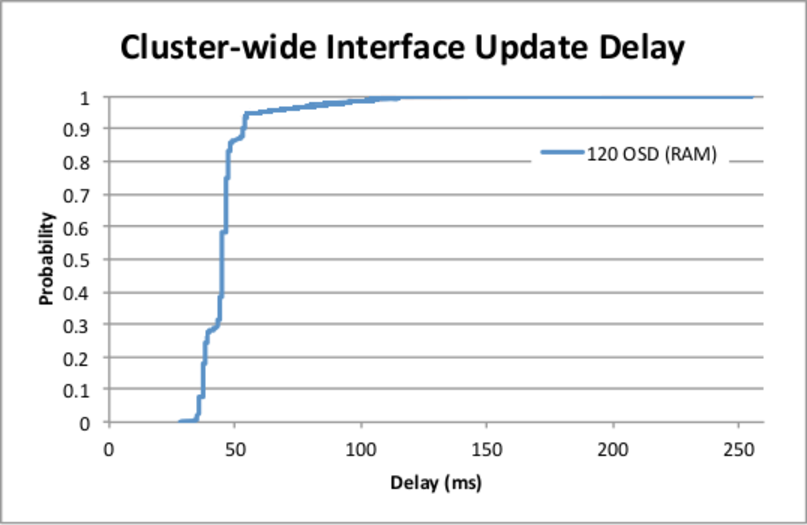
\includegraphics[width=75mm,trim={1 4 4 1.3cm},clip]{figures/iface-update-delay.pdf}
\caption{Cluster-wide interface update latency, excluding the Paxos proposal cost for
interface commit.}
\label{fig:propdelay}
\end{figure}

\subsection{Load Balancing ZLog Sequencers with Mantle}
\label{sec:zlog-balancing}

In practice, a storage system implementing CORFU will support a multiplicity of
independent totally-ordered logs for each application.  For this scenario
co-locating sequencers on the same physical node is not ideal. Building a load
balancer that can migrate the shared resource (in this case, the resource that
mediates access to the tail of the log) is a time-consuming, non-trivial task
that requires building subsystems for migrating resources, monitoring the
workloads, collecting metrics that describe the utilization on the physical
nodes, partitioning resources, maintaining cache coherence, and managing
multiple sequencers. The following experiments demonstrate the feasibility of
using the mechanisms of the Malacology load balancing interface to inherit all
these features and to alleviate load from overloaded servers housing multiple
sequencers.

\begin{figure}[t!]
\centering
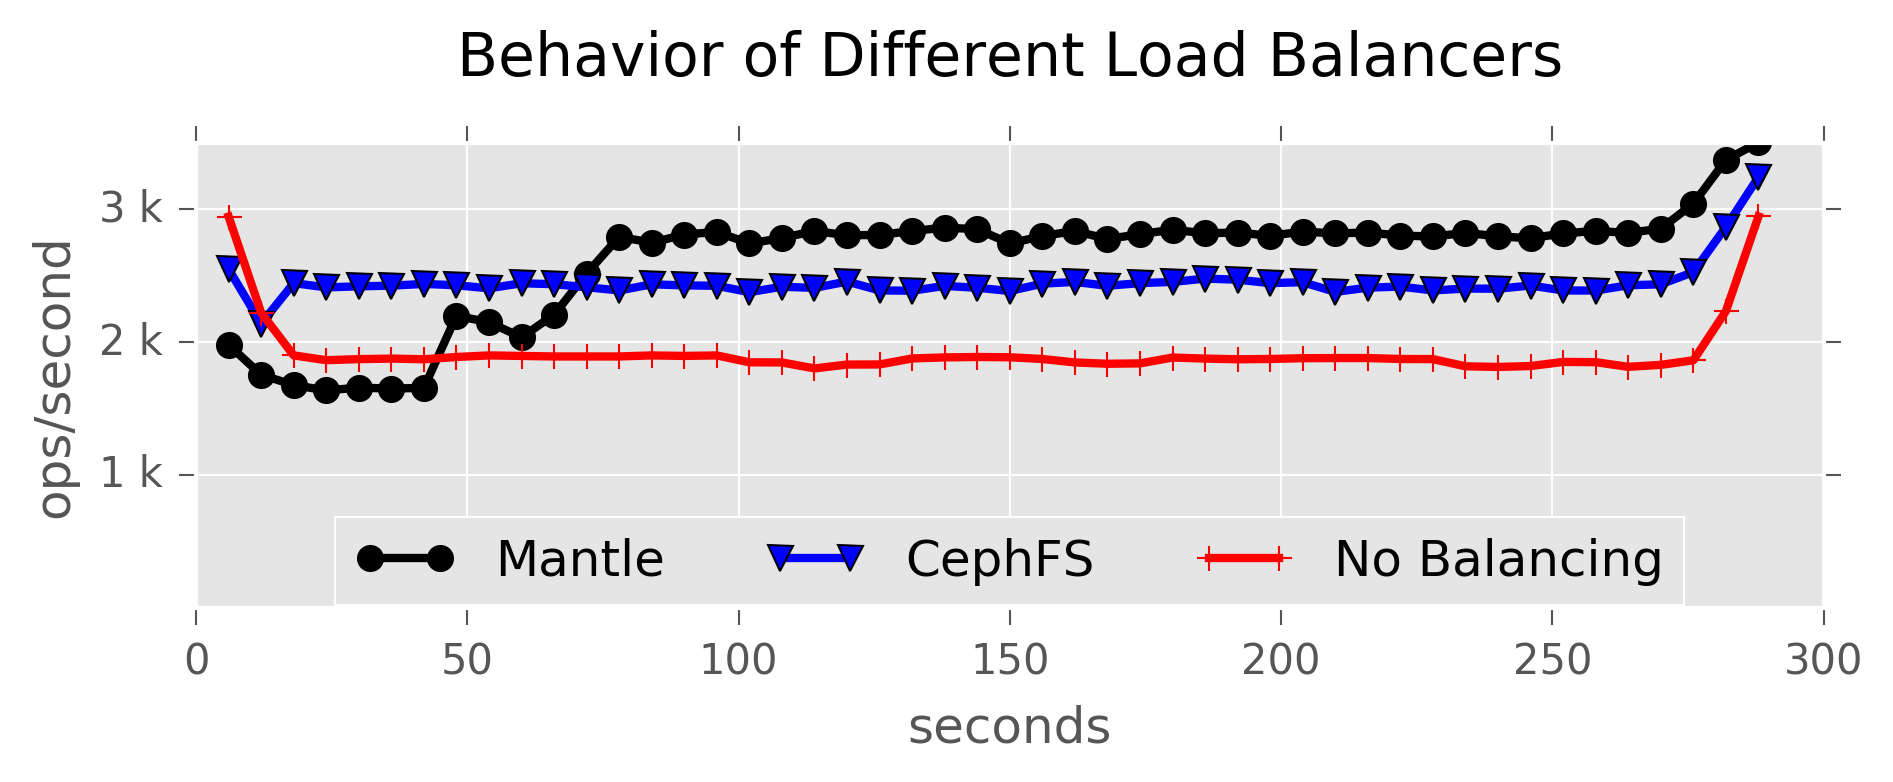
\includegraphics{figures/mantle-balancer-behaviors.png}
\caption{CephFS/Mantle load balancing have better throughput than co-locating
all sequencers on the same server.  Sections~\ref{sec:feature-balancing-modes}
and~\ref{sec:feature-migration-units} quantify this improvement;
Section~\ref{sec:feature-backoff} examines the migration at 0-60 seconds.
}\label{fig:mantle-balancer-behaviors}
\end{figure}

\begin{figure}[t!]
\centering
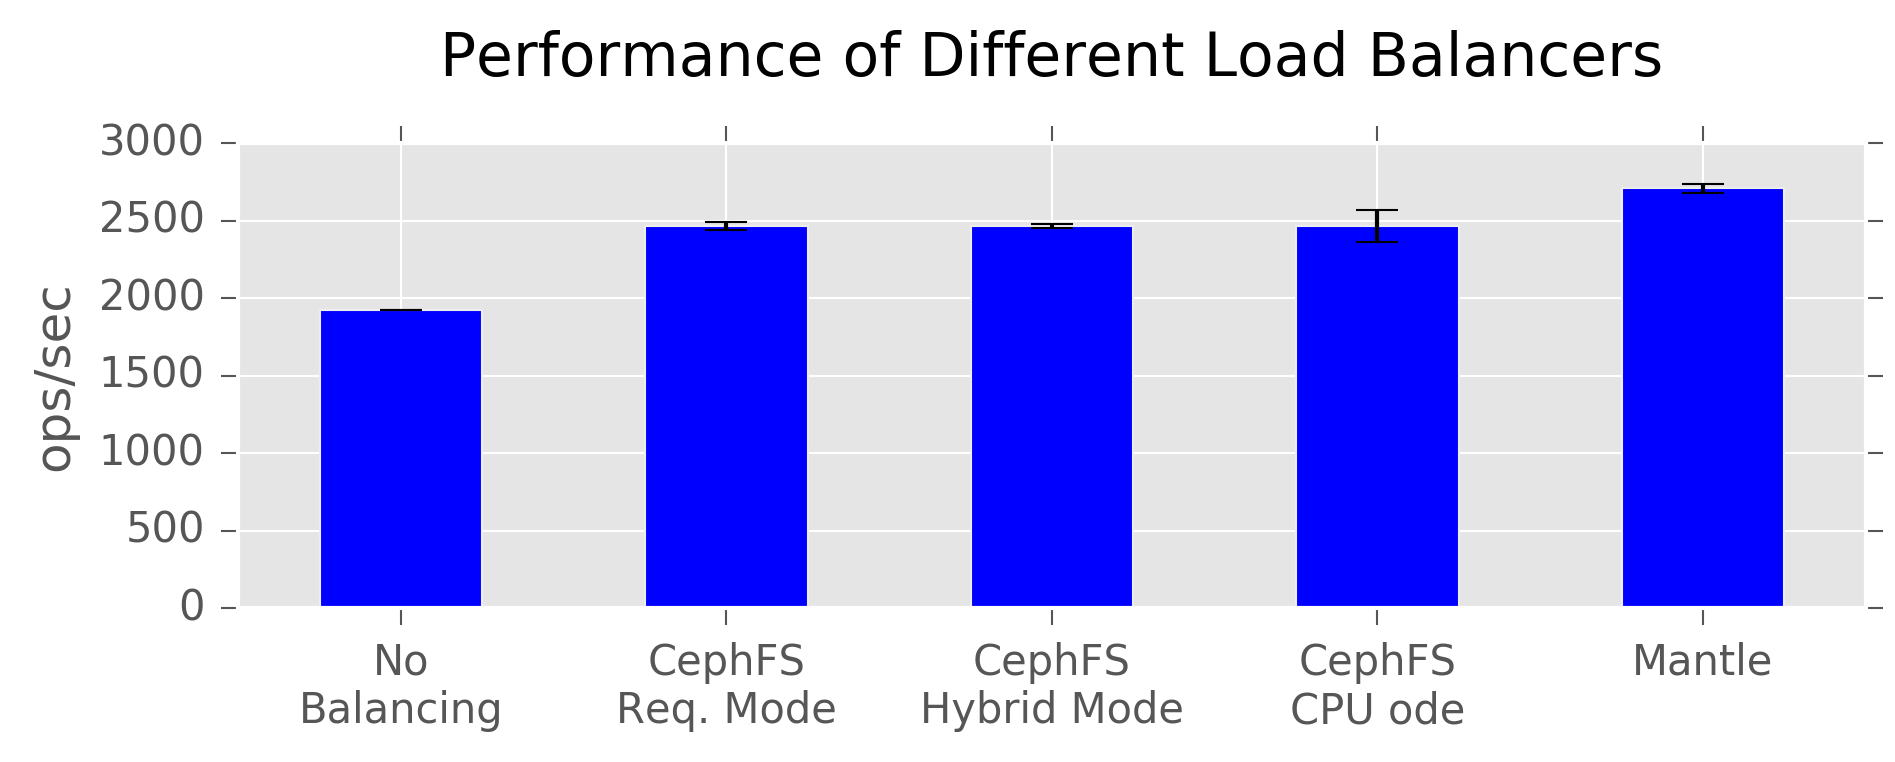
\includegraphics{figures/mantle-balancer-performance.png}
\caption{All CephFS balancing modes have the same performance Mantle uses a
balancer designed for sequencers.}\label{fig:mantle-balancer-performance}
\end{figure}

The experiments are run on a cluster with 10 nodes to store objects, one node
to monitor the cluster, and 3 nodes that can accomodate sequencers. Our first
experiment co-locates 3 sequencers each with 4 clients on the same physical
server.  Instead of measuring contention at the clients like
Section~\ref{sec:sequencer-implementation}, these experiments measure
contention at the sequencers by forcing clients to make round-trips for every
request. We implement this using the shared resource interface that forces
round-trips.  Because the sequencer's only function is to  hand out positions
for the tail of the log, the workload is read-heavy.

First, we show how the ZLog service can orchestrate multiple sequencers in a
cluster using the Malacology load balancing interface.
Figure~\ref{fig:mantle-balancer-behaviors} shows the throughput (\(y\) axis)
over time (\(x\) axis) of different load balancers that migrate ZLog sequencers
acround the cluster; ``No Balancing" keeps all sequencers on one server,
``CephFS" migrates sequencers using the CephFS load balancers, and ``Mantle"
uses a custom load balancer we wrote specifically for sequencers. The CephFS
load balancers are hard-coded into Ceph while Mantle is an API for
balancing load presented in~Mantle~\cite{sevilla:sc15-mantle} and
re-implemented on top of Malacology in this paper.  The increased throughput
for the CephFS and Mantle curves between 0 and 60 seconds are a result of
migrating the sequencer(s) off overloadeed servers.

In addition to showing that migrating sequencers improves performance,
Figure~\ref{fig:mantle-balancer-behaviors} also demonstrates features that we
will explore in the rest of this section.
Sections~\ref{sec:feature-balancing-modes}
and~\ref{sec:feature-migration-units} quantify the differences in performance
when the cluster stabilizes at time 100 seconds and
Section~\ref{sec:feature-backoff} examines the slope and start time of the
rebalancing phase between 0 and 60 seconds by comparing the aggressiveness of
the balancers.

\subsubsection{Feature: Balancing Modes}
\label{sec:feature-balancing-modes}

Next, we quantify the performance benefits shown in
Figure~\ref{fig:mantle-balancer-behaviors}.  To understand why load balancers
perform differently we need to explain the different balancing modes that the
load balancer service uses and how they stress the subsystems that receive and
forward client requests in different ways. In
Figure~\ref{fig:mantle-balancer-behaviors}, the CephFS curve shows the
performance of the balancing mode that CephFS falls into {\it most of the time}.
CephFS has 3 modes for balancing load: CPU mode, workload mode, and hybrid
mode. All three have the same structure for making migration decisions but vary
based on the metric used to calculate load. For this sequencer workload the 3
different modes all have the same performance, shown in
Figure~\ref{fig:mantle-balancer-performance}, because the load balancer falls
into the same mode a majority of the time.  The high variation in performance
for the CephFS CPU Mode bar reflects the uncertainty of using something as
dynamic and unpredictable as CPU utilization to make migration decisions. In
addition to the suboptimal performance and unpredictability, the fact that the
CephFS balancers all fall into the same mode despite using different balancers
is a problem becuase it prevents administrators from properly exploring the
balancing state space.

Mantle gives the administrator more control over the balancing policies; for
the Mantle bar in Figure~\ref{fig:mantle-balancer-performance} we use the load
balancing interface to program logic for balancing read-heavy workloads,
resulting in higher throughput and better stability.  When we did this we also
identified two balancing modes that are relevant for making migration decisions
for sequencers. 

Using Mantle, the administrator can put the load balancing service into ``proxy
mode" or ``client mode". In proxy mode one server receives all requests and
farms off the requests to slave servers; the slaves servers do the actual tail
finding operation. In client mode, clients interact directly with the server
that has their sequencer.  These modes are illustrated in
Figure~\ref{fig:mantle-modes}: ``No balancing" is when all sequencers are
co-located on one physical server -- performance for that mode is shown by the
No Balancing curve in Figure~\ref{fig:mantle-balancer-behaviors}.  ``Client
Mode" in the lower left shows how clients for sequencer 2 are re-directed to
server B. The two ``Proxy mode" diagrams on the right show how clients continue
sending reqeusts to server A even though sequencer 2 has migrated to server B
(the meaning of ``(Half)" is discussed in the next section).

\begin{figure}[t!]
\centering
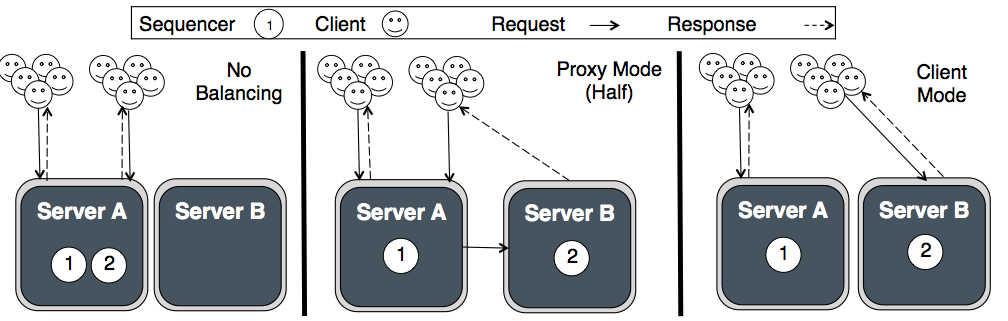
\includegraphics{figures/mantle-modes.png}
\caption{ In client mode clients sending requests to the server that houses
their sequencer. In proxy mode clients continue sending their requests to the
first server.  }\label{fig:mantle-modes}
\end{figure}

\begin{figure}[t!]
\centering
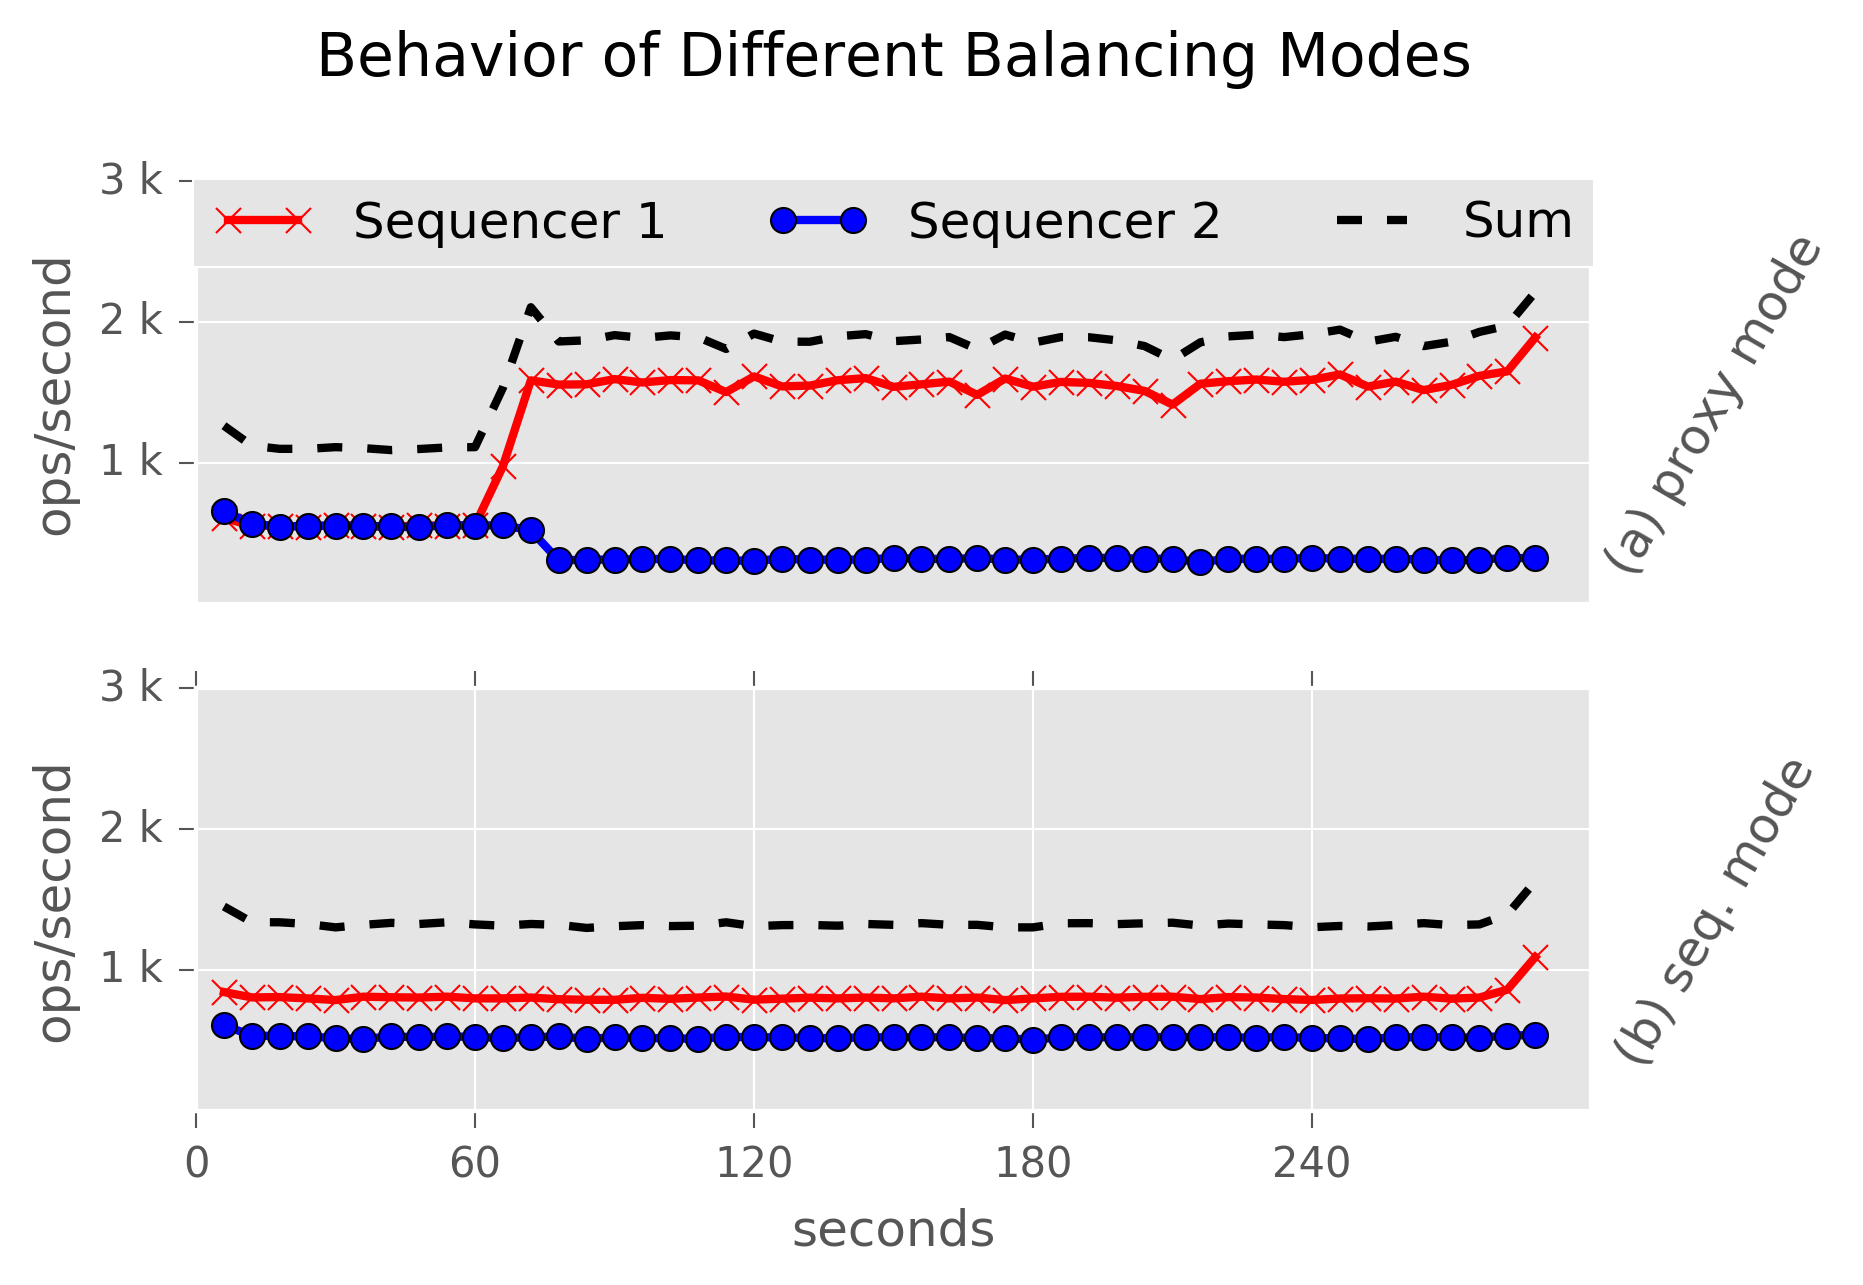
\includegraphics{figures/mantle-mode-behavior.png}
\caption{The performance of proxy mode achieves the highest throughput but at
the cost of lower throughput for one of the sequencers. Client mode is more
fair but results in lower cluster throughput.
}\label{fig:mantle-mode-behavior}
\end{figure}

Figure~\ref{fig:mantle-mode-behavior} shows the throughput over time of the two
different modes for an environment with only 2 sequencers (again 4 clients
each) and 2 servers. The curves for both sequencers in
Figure~\ref{fig:mantle-mode-behavior}(a) start at less than 1000 ops/second and
at time 60 seconds Mantle migrates Sequencer 1 to the slave server.
Performance of Sequencer 2 decreases because it stayed on the proxy which now
handles all client requests, processes requests for Sequencer 2, and forwards
requests for Sequencer 1. The performance of Sequencer 1 improves dramatically
because distributing the sequencers in this way separates (1) the handling of
the client requests and (2) finding the tail of the log and responding to
clients.  Doing both steps is too heavy weight for one server and sequencers on
slave nodes can go faster because work is split up; this phenomenon is not
uncommon and has been observed in chain replication~\cite{CITEME}.  Cluster
throughput improves at the cost of decreased throughput for Sequencer 2.
Figure~\ref{fig:mantle-mode-behavior}(b) is set to sequencer mode manually (no
balancing phase) and shows that the cluster throughput is worse than the
cluster throughput of proxy mode. That graph also shows that Sequencer 2 has
less throughput than Sequencer 2. In this case, the scatter-gather process used
for cache coherence in the metadata protocols causes strain on the server
housing Sequencer 2 resulting in this uneven performance. 

\subsubsection{Feature: Migration Units}
\label{sec:feature-migration-units}

Another factor that affects performance in this environment is ``how much" load
is on each server; these experiments quantify that effect by programming
policies into the load balancing interface to control the amount of load to
migrate. We define migration unit as the amount of load to try and migrate.
For example, it is useful to express migration units as a fraction of the total
load.  Expressing this heuristic is not easily achievable with outward facing
tunable parameters (i.e. system knobs) and so the original CephFS balancers do
not have a migration unit tunable.  With Mantle's programmable interface, we
force the load balancer into the Proxy Mode (Full) scenario in
Figure~\ref{fig:mantle-modes}, which sets the balancer to proxy mode with
migration units equal to the entire load on the current server we can use the Mantle
policy:\\

\noindent \texttt{ targets[\#mds+1] = mds[whoami]["load"] }\\

This code snippet uses globally defined variables and tables from the Mantle
API to send half of the load on the current server (whoami) to the next ranked
server (\#mds + 1); the \texttt{targets} array is a globally defined table that
the balancer uses to do the migrations. Alternatively, to set the mode to the
``Proxy (Half)"` setup in Figure~\ref{fig:mantle-modes} we can divide the right
hand side by 2.

\begin{figure}[t!]
\centering
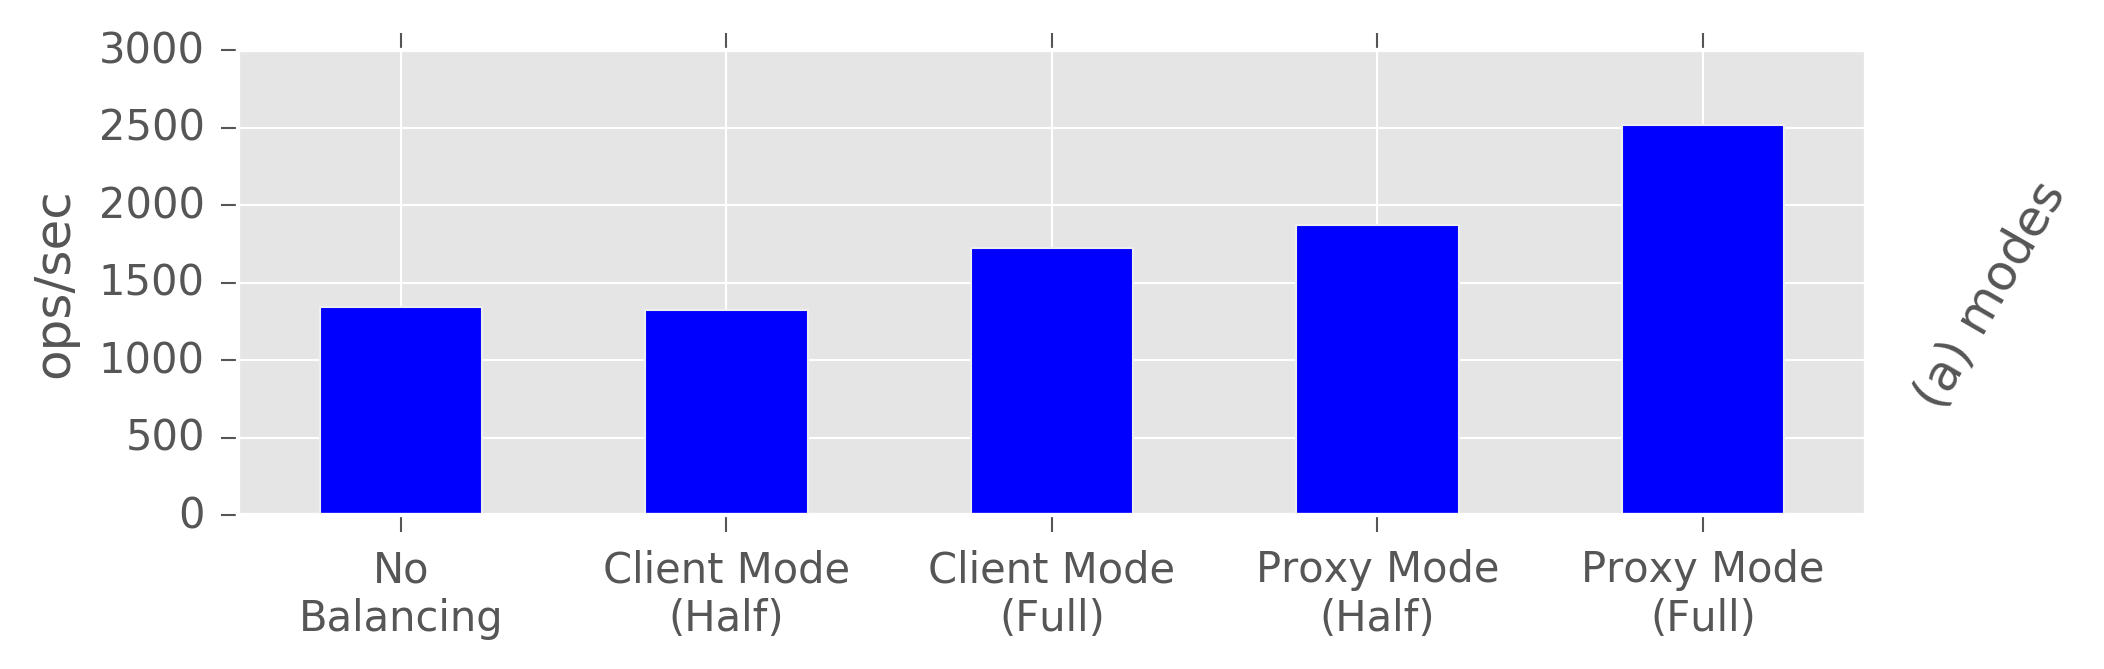
\includegraphics{figures/mantle-mode-performance.png}
\caption{The performance of the different modes using various migration units
shows almost a 2\(\times\) improvement in the best case.
}\label{fig:mantle-mode-performance}
\end{figure}

Figure~\ref{fig:mantle-mode-performance} shows the performance of the modes
using different migration units. Recall that this setup only has 2 sequencers
and 2 servers, so performance may be different at scale. Even so, it is clear
that client mode does not perform as well for read-heavy workloads. We even see
a throughput improvement when migrating all load off the first server, leaving
the first server to do administrative tasks (this is common in the metadata
cluster because the first server does a lot of the cache coherence work) while
the second server does all the client work. Proxy mode does the best in both
cases and shows large performance gains when completely decoupling client
request handling and operation processing in Proxy Mode (Full).  The parameter
that controls the migration units helps the administrator control the sequencer
co-location or distribution across the cluster. This trade-off was explored
extensively in the Mantle paper but the experiments we present here are
indicative of an even richer set of states to explore.

\subsubsection{Feature: Backoff}
\label{sec:feature-backoff}

Tuning the aggressiveness of the load balancer decision making is also a
trade-off that administrators can control and explore. The balancing phase from
0 to 60 seconds in Figure~\ref{fig:mantle-balancer-behaviors} shows different
degrees of aggressiveness in making migration decisions; CephFS makes a
decision quickly and throughput jumps to 2500 ops/second within 10 seconds
while Mantle takes more time to stabilize. This conservative behavior is
controlled by programming the balancer to (1) use different conditions for when
to migrate and (2) using a threshold for sustained overload. 

We control the conditions for migration using \texttt{when()}. \texttt{when()}
is part the Mantle API and the callback expects a return value of true or
false, which corresponds to whether to migrate or not. For the Mantle curve in
Figure~\ref{fig:mantle-balancer-behaviors} we set the \texttt{when()} policy to
wait for load on the receiving server to fall below a threshold. At the
beginning of the run the load of the receiving server spikes because requests
for cache-coherence start as the sequencers are created. It takes 60 seconds
for this load to drop to an acceptable level and it is at this point that the
migration starts.  The Mantle curve in
Figure~\ref{fig:mantle-balancer-behaviors} also takes longer to reach peak
throughput.  This conservative decision making is intentional because we want
the policy wait to see how migrations affect the system before proceeding. The
Mantle curve in Figure~\ref{fig:mantle-balancer-behaviors} does a migration
right before 50 seconds, realizes that there is a third underloaded server, and
does another migration. 

The other way to change aggressiveness of the decision making is to program
into the balancer a threshold for sustatined overload. This forces the balancer
to wait a certain number of iterations after a migration before proceeding. In
Mantle, the policy would use the save state function to do a countdown after a
migation.  Behavior graphs and performance numbers for this backoff feature is
omitted for space considerations, but the throughput graphs are as expected:
the more conservative the approach the less overall throughput.\\
 
\noindent\textbf{Malacology pulls} the load balancing out of the storage system
to balance sequencers across a cluster. Compared to putting all sequencers on
the same server, load balancing a sequencer using the proxy mode shows a
1.8\(\times\) throughput improvement. This latent capability also gives future
programmers the ability to explore the different load balancing trade-offs
including: load balancing modes to control forwarding vs. client redirection,
load migration units to control sequencer distribution vs. co-location, and
backoffs to control conservative vs. aggressive decision making.


%\subsubsection{Experiment: Object Class
%Programmability}\label{experiment-object-class-programmability}
%
%Add quote from CORFU paper that talks about what they had to hack
%
%\subsubsection{Experiment: Multi-Client
%Burstiness}\label{experiment-multi-client-burstiness}
%
%\begin{figure}[htbp] \centering
%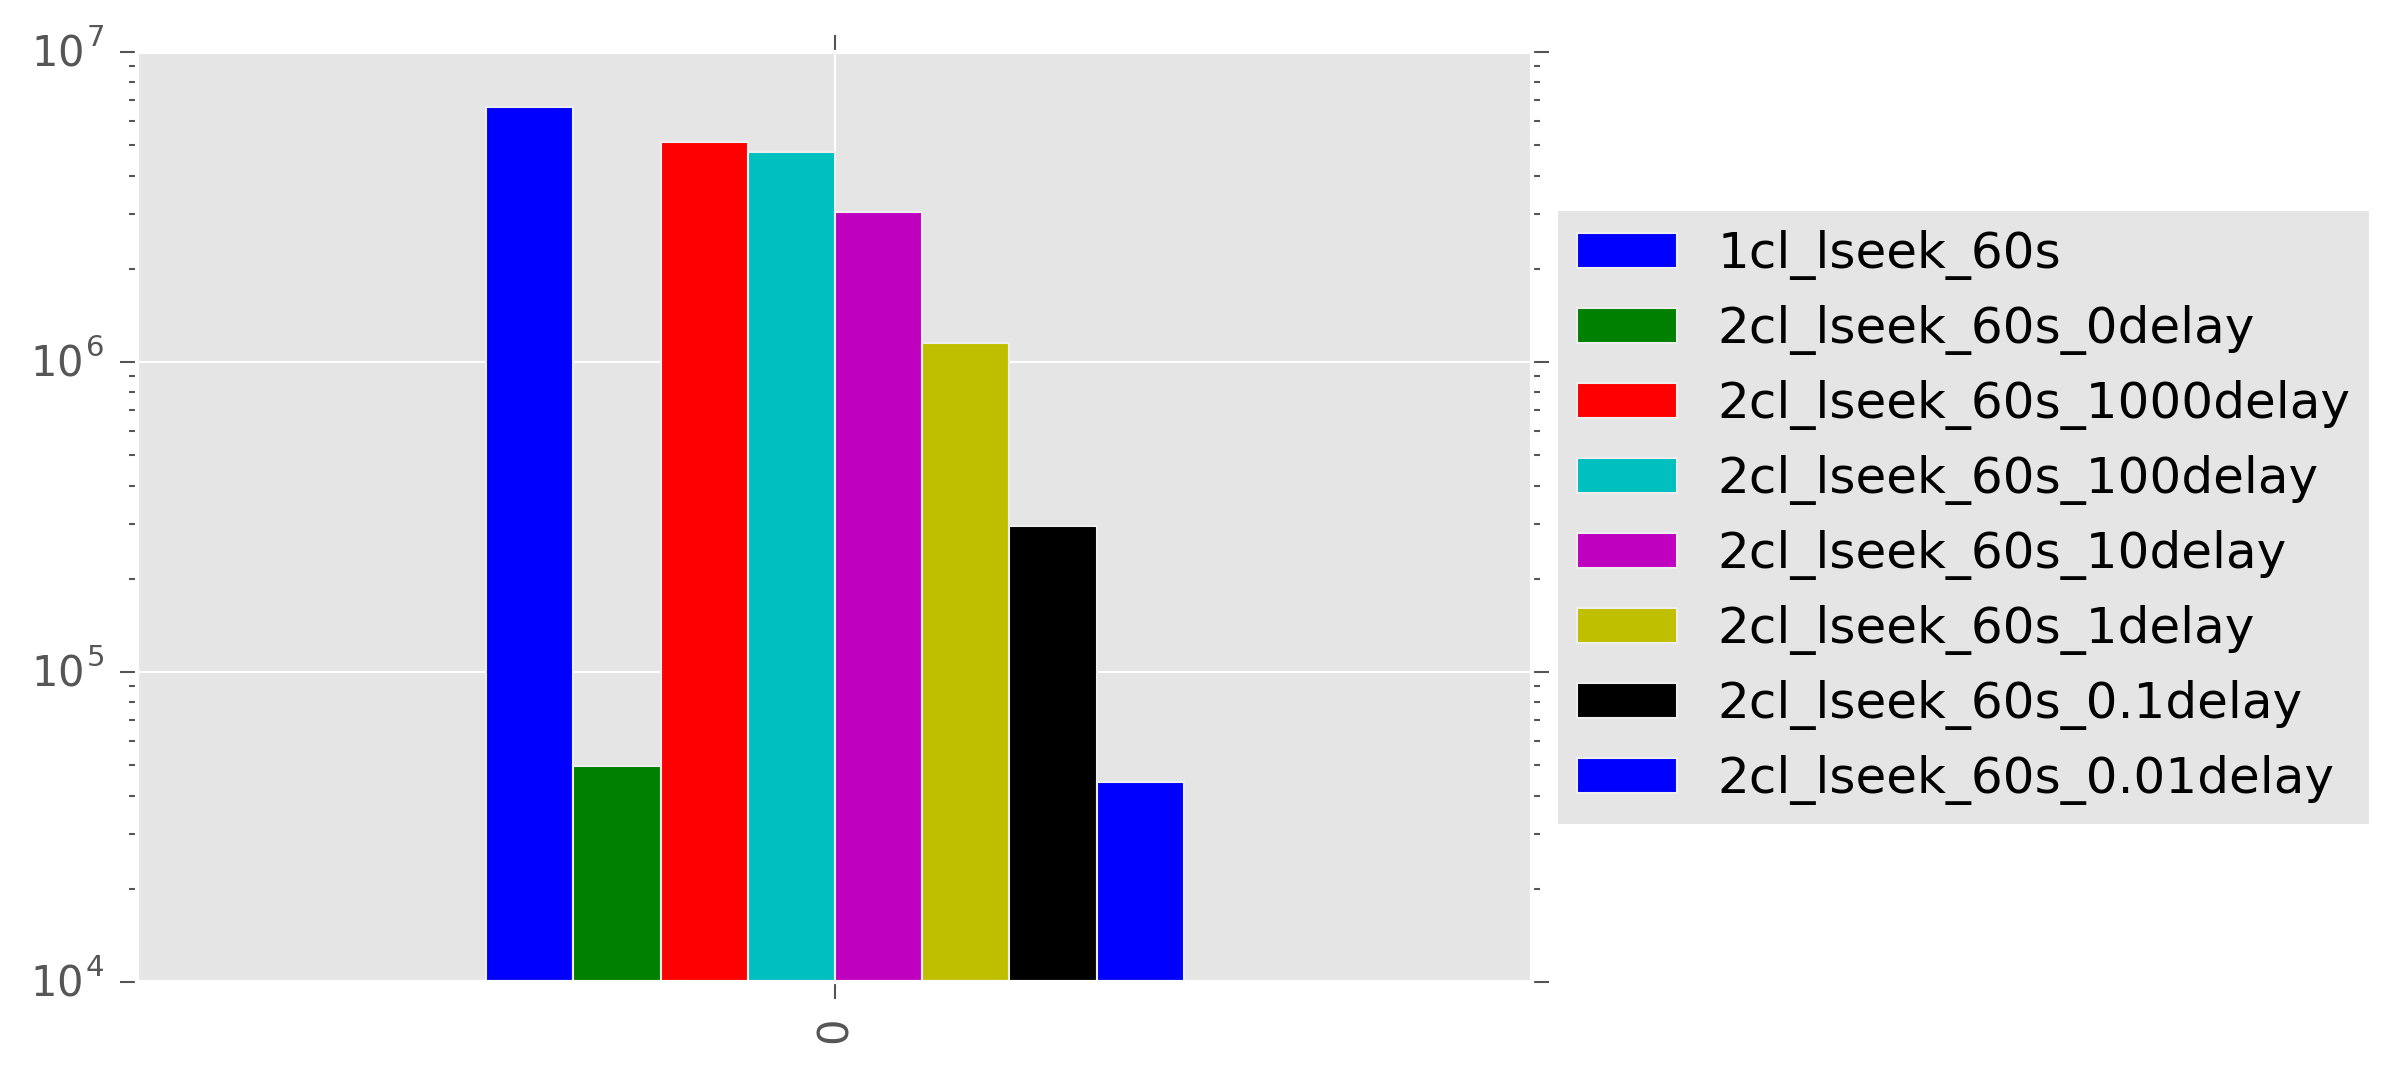
\includegraphics{figures/caps-delay-thruput.png} \caption{Forcing the client
%to drop their capabilities later (delay) improves throughput} \end{figure}

\section{Related Work}

% IOStack: Software-Defined Object Storage
% sRoute: Treating the Storage Stack Like a Network
   % - lots of good refs to check out
% Information and control in gray-box systems

Programmability of operating systems and networking resources, including
distributed storage systems is not new, but we are not aware of work that makes
generalization of existing services into programmable resourses a key principle
in storage systems design. 

Programmable storage systems can be viewed as an infrastructure for creating
abstractions to better separate policies from mechanisms. This idea is not new.
Software-defined networks (SDNs) create such an abstraction by separating the
control plane from the data plane (see for example~\cite{jain:sigcomm13}). This
notion of control/data separation was also applied in software-defined storage
(SDS)~\cite{thereska:sosp13,stefanovici:fast16}. Similarly,
IOStack~\cite{gracia:internet16} is providing policy-based provisioning and
filtering in OpenStack Swift. According to a SNIA white
paper~\cite{carlson:snia2014}, the primary goal of SDS is to control and
facilitate flexible and dynamic provisioning of storage resources of different
kinds, including flash memory and disk drives, to create a virtualized mapping
between common storage abstractions (e.g. files, objects, and blocks) and
storage devices taking data service objectives in terms of protection,
availability, performance, and security into account. A programmable storage
system exposes internal abstractions so that end users (not necessarily
operators) can create new services on top of the storage stack. Thus, our
notion of programmable storage differs from ``software-defined storage'' (SDS)
in terms of goals and scope, although definitions of SDS are still in flux.

Another view of programmable storage systems is one of tailoring systems
resources to applications~\cite{arpaci:sosp01}. Related work includes work
around the Exokernel~\cite{engler:sosp95} and SPIN~\cite{bershad:sosp95} and
Vino~\cite{seltzer:osdi96}, the latter two addressed the ability of injecting
code into the kernel to specialize resource management. Another approach is to
pass hints between the different layers of the IO stack to bridge the semantic
gap between applications and
storage~\cite{arpaci:sosp01,sivathanu:fast03,mesnier:sosp11}).

Malacology uses the same Active and Typed Storage module presented in
DataMods~\cite{watkins_datamods_2012}; Asynchronous Service and File Manifolds
can be implemented with small changes to the Malacology framework, namely
asynchronous object calls and Lua stubs in the inode, respectively.

\section{Conclusion and Future Work}\label{conclusion-and-future-work}

Programmable storage is a viable method for eliminating duplication of complex
error prone software that are used as workarounds for storage system
deficiencies. However, this duplication has real-world problems related to
reliability. We propose that systems expose their services in a safe way
allowing application developers to customize system behavior to meet their
needs while not sacrificing correctness. To illustrate the benefits of this
approach we presented Malacology, a programmable storage system that
facilitates the construction of new services by re-purposing existing subsystem
abstractions of the storage stack.

Future work will focus on constructing more interfaces to support a wide
variety of storage system services that can be configured on-the-fly in existing
systems. This work is one point along that path to producing general-purpose
storage systems that can
target  special-purpose applications.  Ultimately we want to utilize
declarative methods for expressing new services.

\bibliography{paper}
\bibliographystyle{plain}
%\printbibliography

\end{document}
